\documentclass[]{thesis-ekf}
\usepackage[T1]{fontenc}
\PassOptionsToPackage{defaults=hu-min}{magyar.ldf}
\usepackage[magyar]{babel}
\usepackage{mathtools,amssymb,amsthm,pdfpages,listings,multicol,enumitem,wrapfig}
\footnotestyle{rule=fourth}

\newtheorem{tetel}{Tétel}[chapter]
\theoremstyle{definition}
\newtheorem{definicio}[tetel]{Definíció}
\theoremstyle{remark}
\newtheorem{megjegyzes}[tetel]{Megjegyzés}
 %%%%%%%%%%%%%%%%%%%%%%%%%%%%%%%%%%%%%%%%%%%%%%%%%%%%%%%%%%%%%%%%%%%%%%%%%%%%%%%% 
%%% ~ Arduino Language - Arduino IDE Colors ~                                  %%%
%%%                                                                            %%%
%%% Kyle Rocha-Brownell | 10/2/2017 | No Licence                               %%%
%%% -------------------------------------------------------------------------- %%%
%%%                                                                            %%%
%%% Place this file in your working directory (next to the latex file you're   %%%
%%% working on).  To add it to your project, place:                            %%%
%%%     %%%%%%%%%%%%%%%%%%%%%%%%%%%%%%%%%%%%%%%%%%%%%%%%%%%%%%%%%%%%%%%%%%%%%%%%%%%%%%%% 
%%% ~ Arduino Language - Arduino IDE Colors ~                                  %%%
%%%                                                                            %%%
%%% Kyle Rocha-Brownell | 10/2/2017 | No Licence                               %%%
%%% -------------------------------------------------------------------------- %%%
%%%                                                                            %%%
%%% Place this file in your working directory (next to the latex file you're   %%%
%%% working on).  To add it to your project, place:                            %%%
%%%     %%%%%%%%%%%%%%%%%%%%%%%%%%%%%%%%%%%%%%%%%%%%%%%%%%%%%%%%%%%%%%%%%%%%%%%%%%%%%%%% 
%%% ~ Arduino Language - Arduino IDE Colors ~                                  %%%
%%%                                                                            %%%
%%% Kyle Rocha-Brownell | 10/2/2017 | No Licence                               %%%
%%% -------------------------------------------------------------------------- %%%
%%%                                                                            %%%
%%% Place this file in your working directory (next to the latex file you're   %%%
%%% working on).  To add it to your project, place:                            %%%
%%%    \input{arduinoLanguage.tex}                                             %%%
%%% somewhere before \begin{document} in your latex file.                      %%%
%%%                                                                            %%%
%%% In your document, place your arduino code between:                         %%%
%%%   \begin{lstlisting}[language=Arduino]                                     %%%
%%% and:                                                                       %%%
%%%   \end{lstlisting}                                                         %%%
%%%                                                                            %%%
%%% Or create your own style to add non-built-in functions and variables.      %%%
%%%                                                                            %%%
 %%%%%%%%%%%%%%%%%%%%%%%%%%%%%%%%%%%%%%%%%%%%%%%%%%%%%%%%%%%%%%%%%%%%%%%%%%%%%%%% 

\usepackage{color}
\usepackage{listings}    
\usepackage{courier}

%%% Define Custom IDE Colors %%%
\definecolor{arduinoGreen}    {rgb} {0.17, 0.43, 0.01}
\definecolor{arduinoGrey}     {rgb} {0.47, 0.47, 0.33}
\definecolor{arduinoOrange}   {rgb} {0.8 , 0.4 , 0   }
\definecolor{arduinoBlue}     {rgb} {0.01, 0.61, 0.98}
\definecolor{arduinoDarkBlue} {rgb} {0.0 , 0.2 , 0.5 }

%%% Define Arduino Language %%%
\lstdefinelanguage{Arduino}{
  language=C++, % begin with default C++ settings 
%
%
  %%% Keyword Color Group 1 %%%  (called KEYWORD3 by arduino)
  keywordstyle=\color{arduinoGreen},   
  deletekeywords={  % remove all arduino keywords that might be in c++
                break, case, override, final, continue, default, do, else, for, 
                if, return, goto, switch, throw, try, while, setup, loop, export, 
                not, or, and, xor, include, define, elif, else, error, if, ifdef, 
                ifndef, pragma, warning,
                HIGH, LOW, INPUT, INPUT_PULLUP, OUTPUT, DEC, BIN, HEX, OCT, PI, 
                HALF_PI, TWO_PI, LSBFIRST, MSBFIRST, CHANGE, FALLING, RISING, 
                DEFAULT, EXTERNAL, INTERNAL, INTERNAL1V1, INTERNAL2V56, LED_BUILTIN, 
                LED_BUILTIN_RX, LED_BUILTIN_TX, DIGITAL_MESSAGE, FIRMATA_STRING, 
                ANALOG_MESSAGE, REPORT_DIGITAL, REPORT_ANALOG, SET_PIN_MODE, 
                SYSTEM_RESET, SYSEX_START, auto, int8_t, int16_t, int32_t, int64_t, 
                uint8_t, uint16_t, uint32_t, uint64_t, char16_t, char32_t, operator, 
                enum, delete, bool, boolean, byte, char, const, false, float, double, 
                null, NULL, int, long, new, private, protected, public, short, 
                signed, static, volatile, String, void, true, unsigned, word, array, 
                sizeof, dynamic_cast, typedef, const_cast, struct, static_cast, union, 
                friend, extern, class, reinterpret_cast, register, explicit, inline, 
                _Bool, complex, _Complex, _Imaginary, atomic_bool, atomic_char, 
                atomic_schar, atomic_uchar, atomic_short, atomic_ushort, atomic_int, 
                atomic_uint, atomic_long, atomic_ulong, atomic_llong, atomic_ullong, 
                virtual, PROGMEM,
                Serial, Serial1, Serial2, Serial3, SerialUSB, Keyboard, Mouse,
                abs, acos, asin, atan, atan2, ceil, constrain, cos, degrees, exp, 
                floor, log, map, max, min, radians, random, randomSeed, round, sin, 
                sq, sqrt, tan, pow, bitRead, bitWrite, bitSet, bitClear, bit, 
                highByte, lowByte, analogReference, analogRead, 
                analogReadResolution, analogWrite, analogWriteResolution, 
                attachInterrupt, detachInterrupt, digitalPinToInterrupt, delay, 
                delayMicroseconds, digitalWrite, digitalRead, interrupts, millis, 
                micros, noInterrupts, noTone, pinMode, pulseIn, pulseInLong, shiftIn, 
                shiftOut, tone, yield, Stream, begin, end, peek, read, print, 
                println, available, availableForWrite, flush, setTimeout, find, 
                findUntil, parseInt, parseFloat, readBytes, readBytesUntil, readString, 
                readStringUntil, trim, toUpperCase, toLowerCase, charAt, compareTo, 
                concat, endsWith, startsWith, equals, equalsIgnoreCase, getBytes, 
                indexOf, lastIndexOf, length, replace, setCharAt, substring, 
                toCharArray, toInt, press, release, releaseAll, accept, click, move, 
                isPressed, isAlphaNumeric, isAlpha, isAscii, isWhitespace, isControl, 
                isDigit, isGraph, isLowerCase, isPrintable, isPunct, isSpace, 
                isUpperCase, isHexadecimalDigit, 
                }, 
  morekeywords={   % add arduino structures to group 1
                break, case, override, final, continue, default, do, else, for, 
                if, return, goto, switch, throw, try, while, setup, loop, export, 
                not, or, and, xor, include, define, elif, else, error, if, ifdef, 
                ifndef, pragma, warning,
                }, 
% 
%
  %%% Keyword Color Group 2 %%%  (called LITERAL1 by arduino)
  keywordstyle=[2]\color{arduinoBlue},   
  keywords=[2]{   % add variables and dataTypes as 2nd group  
                HIGH, LOW, INPUT, INPUT_PULLUP, OUTPUT, DEC, BIN, HEX, OCT, PI, 
                HALF_PI, TWO_PI, LSBFIRST, MSBFIRST, CHANGE, FALLING, RISING, 
                DEFAULT, EXTERNAL, INTERNAL, INTERNAL1V1, INTERNAL2V56, LED_BUILTIN, 
                LED_BUILTIN_RX, LED_BUILTIN_TX, DIGITAL_MESSAGE, FIRMATA_STRING, 
                ANALOG_MESSAGE, REPORT_DIGITAL, REPORT_ANALOG, SET_PIN_MODE, 
                SYSTEM_RESET, SYSEX_START, auto, int8_t, int16_t, int32_t, int64_t, 
                uint8_t, uint16_t, uint32_t, uint64_t, char16_t, char32_t, operator, 
                enum, delete, bool, boolean, byte, char, const, false, float, double, 
                null, NULL, int, long, new, private, protected, public, short, 
                signed, static, volatile, String, void, true, unsigned, word, array, 
                sizeof, dynamic_cast, typedef, const_cast, struct, static_cast, union, 
                friend, extern, class, reinterpret_cast, register, explicit, inline, 
                _Bool, complex, _Complex, _Imaginary, atomic_bool, atomic_char, 
                atomic_schar, atomic_uchar, atomic_short, atomic_ushort, atomic_int, 
                atomic_uint, atomic_long, atomic_ulong, atomic_llong, atomic_ullong, 
                virtual, PROGMEM,
                },  
% 
%
  %%% Keyword Color Group 3 %%%  (called KEYWORD1 by arduino)
  keywordstyle=[3]\bfseries\color{arduinoOrange},
  keywords=[3]{  % add built-in functions as a 3rd group
                Serial, Serial1, Serial2, Serial3, SerialUSB, Keyboard, Mouse,
                },      
%
%
  %%% Keyword Color Group 4 %%%  (called KEYWORD2 by arduino)
  keywordstyle=[4]\color{arduinoOrange},
  keywords=[4]{  % add more built-in functions as a 4th group
                abs, acos, asin, atan, atan2, ceil, constrain, cos, degrees, exp, 
                floor, log, map, max, min, radians, random, randomSeed, round, sin, 
                sq, sqrt, tan, pow, bitRead, bitWrite, bitSet, bitClear, bit, 
                highByte, lowByte, analogReference, analogRead, 
                analogReadResolution, analogWrite, analogWriteResolution, 
                attachInterrupt, detachInterrupt, digitalPinToInterrupt, delay, 
                delayMicroseconds, digitalWrite, digitalRead, interrupts, millis, 
                micros, noInterrupts, noTone, pinMode, pulseIn, pulseInLong, shiftIn, 
                shiftOut, tone, yield, Stream, begin, end, peek, read, print, 
                println, available, availableForWrite, flush, setTimeout, find, 
                findUntil, parseInt, parseFloat, readBytes, readBytesUntil, readString, 
                readStringUntil, trim, toUpperCase, toLowerCase, charAt, compareTo, 
                concat, endsWith, startsWith, equals, equalsIgnoreCase, getBytes, 
                indexOf, lastIndexOf, length, replace, setCharAt, substring, 
                toCharArray, toInt, press, release, releaseAll, accept, click, move, 
                isPressed, isAlphaNumeric, isAlpha, isAscii, isWhitespace, isControl, 
                isDigit, isGraph, isLowerCase, isPrintable, isPunct, isSpace, 
                isUpperCase, isHexadecimalDigit,
                adns_write_reg,adns_com_begin,SPI,transfer,adns_com_end
                },      
%
%
  %%% Set Other Colors %%%
  stringstyle=\color{arduinoDarkBlue},    
  commentstyle=\color{arduinoGrey},    
%          
%   
  %%%% Line Numbering %%%%
  numbers=left,                    
  numbersep=5pt,                   
  numberstyle=\color{arduinoGrey},    
  %stepnumber=2,                      % show every 2 line numbers
%
%
  %%%% Code Box Style %%%%
  breaklines=true,                    % wordwrapping
  tabsize=2,         
  basicstyle=\ttfamily  
}
                                             %%%
%%% somewhere before \begin{document} in your latex file.                      %%%
%%%                                                                            %%%
%%% In your document, place your arduino code between:                         %%%
%%%   \begin{lstlisting}[language=Arduino]                                     %%%
%%% and:                                                                       %%%
%%%   \end{lstlisting}                                                         %%%
%%%                                                                            %%%
%%% Or create your own style to add non-built-in functions and variables.      %%%
%%%                                                                            %%%
 %%%%%%%%%%%%%%%%%%%%%%%%%%%%%%%%%%%%%%%%%%%%%%%%%%%%%%%%%%%%%%%%%%%%%%%%%%%%%%%% 

\usepackage{color}
\usepackage{listings}    
\usepackage{courier}

%%% Define Custom IDE Colors %%%
\definecolor{arduinoGreen}    {rgb} {0.17, 0.43, 0.01}
\definecolor{arduinoGrey}     {rgb} {0.47, 0.47, 0.33}
\definecolor{arduinoOrange}   {rgb} {0.8 , 0.4 , 0   }
\definecolor{arduinoBlue}     {rgb} {0.01, 0.61, 0.98}
\definecolor{arduinoDarkBlue} {rgb} {0.0 , 0.2 , 0.5 }

%%% Define Arduino Language %%%
\lstdefinelanguage{Arduino}{
  language=C++, % begin with default C++ settings 
%
%
  %%% Keyword Color Group 1 %%%  (called KEYWORD3 by arduino)
  keywordstyle=\color{arduinoGreen},   
  deletekeywords={  % remove all arduino keywords that might be in c++
                break, case, override, final, continue, default, do, else, for, 
                if, return, goto, switch, throw, try, while, setup, loop, export, 
                not, or, and, xor, include, define, elif, else, error, if, ifdef, 
                ifndef, pragma, warning,
                HIGH, LOW, INPUT, INPUT_PULLUP, OUTPUT, DEC, BIN, HEX, OCT, PI, 
                HALF_PI, TWO_PI, LSBFIRST, MSBFIRST, CHANGE, FALLING, RISING, 
                DEFAULT, EXTERNAL, INTERNAL, INTERNAL1V1, INTERNAL2V56, LED_BUILTIN, 
                LED_BUILTIN_RX, LED_BUILTIN_TX, DIGITAL_MESSAGE, FIRMATA_STRING, 
                ANALOG_MESSAGE, REPORT_DIGITAL, REPORT_ANALOG, SET_PIN_MODE, 
                SYSTEM_RESET, SYSEX_START, auto, int8_t, int16_t, int32_t, int64_t, 
                uint8_t, uint16_t, uint32_t, uint64_t, char16_t, char32_t, operator, 
                enum, delete, bool, boolean, byte, char, const, false, float, double, 
                null, NULL, int, long, new, private, protected, public, short, 
                signed, static, volatile, String, void, true, unsigned, word, array, 
                sizeof, dynamic_cast, typedef, const_cast, struct, static_cast, union, 
                friend, extern, class, reinterpret_cast, register, explicit, inline, 
                _Bool, complex, _Complex, _Imaginary, atomic_bool, atomic_char, 
                atomic_schar, atomic_uchar, atomic_short, atomic_ushort, atomic_int, 
                atomic_uint, atomic_long, atomic_ulong, atomic_llong, atomic_ullong, 
                virtual, PROGMEM,
                Serial, Serial1, Serial2, Serial3, SerialUSB, Keyboard, Mouse,
                abs, acos, asin, atan, atan2, ceil, constrain, cos, degrees, exp, 
                floor, log, map, max, min, radians, random, randomSeed, round, sin, 
                sq, sqrt, tan, pow, bitRead, bitWrite, bitSet, bitClear, bit, 
                highByte, lowByte, analogReference, analogRead, 
                analogReadResolution, analogWrite, analogWriteResolution, 
                attachInterrupt, detachInterrupt, digitalPinToInterrupt, delay, 
                delayMicroseconds, digitalWrite, digitalRead, interrupts, millis, 
                micros, noInterrupts, noTone, pinMode, pulseIn, pulseInLong, shiftIn, 
                shiftOut, tone, yield, Stream, begin, end, peek, read, print, 
                println, available, availableForWrite, flush, setTimeout, find, 
                findUntil, parseInt, parseFloat, readBytes, readBytesUntil, readString, 
                readStringUntil, trim, toUpperCase, toLowerCase, charAt, compareTo, 
                concat, endsWith, startsWith, equals, equalsIgnoreCase, getBytes, 
                indexOf, lastIndexOf, length, replace, setCharAt, substring, 
                toCharArray, toInt, press, release, releaseAll, accept, click, move, 
                isPressed, isAlphaNumeric, isAlpha, isAscii, isWhitespace, isControl, 
                isDigit, isGraph, isLowerCase, isPrintable, isPunct, isSpace, 
                isUpperCase, isHexadecimalDigit, 
                }, 
  morekeywords={   % add arduino structures to group 1
                break, case, override, final, continue, default, do, else, for, 
                if, return, goto, switch, throw, try, while, setup, loop, export, 
                not, or, and, xor, include, define, elif, else, error, if, ifdef, 
                ifndef, pragma, warning,
                }, 
% 
%
  %%% Keyword Color Group 2 %%%  (called LITERAL1 by arduino)
  keywordstyle=[2]\color{arduinoBlue},   
  keywords=[2]{   % add variables and dataTypes as 2nd group  
                HIGH, LOW, INPUT, INPUT_PULLUP, OUTPUT, DEC, BIN, HEX, OCT, PI, 
                HALF_PI, TWO_PI, LSBFIRST, MSBFIRST, CHANGE, FALLING, RISING, 
                DEFAULT, EXTERNAL, INTERNAL, INTERNAL1V1, INTERNAL2V56, LED_BUILTIN, 
                LED_BUILTIN_RX, LED_BUILTIN_TX, DIGITAL_MESSAGE, FIRMATA_STRING, 
                ANALOG_MESSAGE, REPORT_DIGITAL, REPORT_ANALOG, SET_PIN_MODE, 
                SYSTEM_RESET, SYSEX_START, auto, int8_t, int16_t, int32_t, int64_t, 
                uint8_t, uint16_t, uint32_t, uint64_t, char16_t, char32_t, operator, 
                enum, delete, bool, boolean, byte, char, const, false, float, double, 
                null, NULL, int, long, new, private, protected, public, short, 
                signed, static, volatile, String, void, true, unsigned, word, array, 
                sizeof, dynamic_cast, typedef, const_cast, struct, static_cast, union, 
                friend, extern, class, reinterpret_cast, register, explicit, inline, 
                _Bool, complex, _Complex, _Imaginary, atomic_bool, atomic_char, 
                atomic_schar, atomic_uchar, atomic_short, atomic_ushort, atomic_int, 
                atomic_uint, atomic_long, atomic_ulong, atomic_llong, atomic_ullong, 
                virtual, PROGMEM,
                },  
% 
%
  %%% Keyword Color Group 3 %%%  (called KEYWORD1 by arduino)
  keywordstyle=[3]\bfseries\color{arduinoOrange},
  keywords=[3]{  % add built-in functions as a 3rd group
                Serial, Serial1, Serial2, Serial3, SerialUSB, Keyboard, Mouse,
                },      
%
%
  %%% Keyword Color Group 4 %%%  (called KEYWORD2 by arduino)
  keywordstyle=[4]\color{arduinoOrange},
  keywords=[4]{  % add more built-in functions as a 4th group
                abs, acos, asin, atan, atan2, ceil, constrain, cos, degrees, exp, 
                floor, log, map, max, min, radians, random, randomSeed, round, sin, 
                sq, sqrt, tan, pow, bitRead, bitWrite, bitSet, bitClear, bit, 
                highByte, lowByte, analogReference, analogRead, 
                analogReadResolution, analogWrite, analogWriteResolution, 
                attachInterrupt, detachInterrupt, digitalPinToInterrupt, delay, 
                delayMicroseconds, digitalWrite, digitalRead, interrupts, millis, 
                micros, noInterrupts, noTone, pinMode, pulseIn, pulseInLong, shiftIn, 
                shiftOut, tone, yield, Stream, begin, end, peek, read, print, 
                println, available, availableForWrite, flush, setTimeout, find, 
                findUntil, parseInt, parseFloat, readBytes, readBytesUntil, readString, 
                readStringUntil, trim, toUpperCase, toLowerCase, charAt, compareTo, 
                concat, endsWith, startsWith, equals, equalsIgnoreCase, getBytes, 
                indexOf, lastIndexOf, length, replace, setCharAt, substring, 
                toCharArray, toInt, press, release, releaseAll, accept, click, move, 
                isPressed, isAlphaNumeric, isAlpha, isAscii, isWhitespace, isControl, 
                isDigit, isGraph, isLowerCase, isPrintable, isPunct, isSpace, 
                isUpperCase, isHexadecimalDigit,
                adns_write_reg,adns_com_begin,SPI,transfer,adns_com_end
                },      
%
%
  %%% Set Other Colors %%%
  stringstyle=\color{arduinoDarkBlue},    
  commentstyle=\color{arduinoGrey},    
%          
%   
  %%%% Line Numbering %%%%
  numbers=left,                    
  numbersep=5pt,                   
  numberstyle=\color{arduinoGrey},    
  %stepnumber=2,                      % show every 2 line numbers
%
%
  %%%% Code Box Style %%%%
  breaklines=true,                    % wordwrapping
  tabsize=2,         
  basicstyle=\ttfamily  
}
                                             %%%
%%% somewhere before \begin{document} in your latex file.                      %%%
%%%                                                                            %%%
%%% In your document, place your arduino code between:                         %%%
%%%   \begin{lstlisting}[language=Arduino]                                     %%%
%%% and:                                                                       %%%
%%%   \end{lstlisting}                                                         %%%
%%%                                                                            %%%
%%% Or create your own style to add non-built-in functions and variables.      %%%
%%%                                                                            %%%
 %%%%%%%%%%%%%%%%%%%%%%%%%%%%%%%%%%%%%%%%%%%%%%%%%%%%%%%%%%%%%%%%%%%%%%%%%%%%%%%% 

\usepackage{color}
\usepackage{listings}    
\usepackage{courier}

%%% Define Custom IDE Colors %%%
\definecolor{arduinoGreen}    {rgb} {0.17, 0.43, 0.01}
\definecolor{arduinoGrey}     {rgb} {0.47, 0.47, 0.33}
\definecolor{arduinoOrange}   {rgb} {0.8 , 0.4 , 0   }
\definecolor{arduinoBlue}     {rgb} {0.01, 0.61, 0.98}
\definecolor{arduinoDarkBlue} {rgb} {0.0 , 0.2 , 0.5 }

%%% Define Arduino Language %%%
\lstdefinelanguage{Arduino}{
  language=C++, % begin with default C++ settings 
%
%
  %%% Keyword Color Group 1 %%%  (called KEYWORD3 by arduino)
  keywordstyle=\color{arduinoGreen},   
  deletekeywords={  % remove all arduino keywords that might be in c++
                break, case, override, final, continue, default, do, else, for, 
                if, return, goto, switch, throw, try, while, setup, loop, export, 
                not, or, and, xor, include, define, elif, else, error, if, ifdef, 
                ifndef, pragma, warning,
                HIGH, LOW, INPUT, INPUT_PULLUP, OUTPUT, DEC, BIN, HEX, OCT, PI, 
                HALF_PI, TWO_PI, LSBFIRST, MSBFIRST, CHANGE, FALLING, RISING, 
                DEFAULT, EXTERNAL, INTERNAL, INTERNAL1V1, INTERNAL2V56, LED_BUILTIN, 
                LED_BUILTIN_RX, LED_BUILTIN_TX, DIGITAL_MESSAGE, FIRMATA_STRING, 
                ANALOG_MESSAGE, REPORT_DIGITAL, REPORT_ANALOG, SET_PIN_MODE, 
                SYSTEM_RESET, SYSEX_START, auto, int8_t, int16_t, int32_t, int64_t, 
                uint8_t, uint16_t, uint32_t, uint64_t, char16_t, char32_t, operator, 
                enum, delete, bool, boolean, byte, char, const, false, float, double, 
                null, NULL, int, long, new, private, protected, public, short, 
                signed, static, volatile, String, void, true, unsigned, word, array, 
                sizeof, dynamic_cast, typedef, const_cast, struct, static_cast, union, 
                friend, extern, class, reinterpret_cast, register, explicit, inline, 
                _Bool, complex, _Complex, _Imaginary, atomic_bool, atomic_char, 
                atomic_schar, atomic_uchar, atomic_short, atomic_ushort, atomic_int, 
                atomic_uint, atomic_long, atomic_ulong, atomic_llong, atomic_ullong, 
                virtual, PROGMEM,
                Serial, Serial1, Serial2, Serial3, SerialUSB, Keyboard, Mouse,
                abs, acos, asin, atan, atan2, ceil, constrain, cos, degrees, exp, 
                floor, log, map, max, min, radians, random, randomSeed, round, sin, 
                sq, sqrt, tan, pow, bitRead, bitWrite, bitSet, bitClear, bit, 
                highByte, lowByte, analogReference, analogRead, 
                analogReadResolution, analogWrite, analogWriteResolution, 
                attachInterrupt, detachInterrupt, digitalPinToInterrupt, delay, 
                delayMicroseconds, digitalWrite, digitalRead, interrupts, millis, 
                micros, noInterrupts, noTone, pinMode, pulseIn, pulseInLong, shiftIn, 
                shiftOut, tone, yield, Stream, begin, end, peek, read, print, 
                println, available, availableForWrite, flush, setTimeout, find, 
                findUntil, parseInt, parseFloat, readBytes, readBytesUntil, readString, 
                readStringUntil, trim, toUpperCase, toLowerCase, charAt, compareTo, 
                concat, endsWith, startsWith, equals, equalsIgnoreCase, getBytes, 
                indexOf, lastIndexOf, length, replace, setCharAt, substring, 
                toCharArray, toInt, press, release, releaseAll, accept, click, move, 
                isPressed, isAlphaNumeric, isAlpha, isAscii, isWhitespace, isControl, 
                isDigit, isGraph, isLowerCase, isPrintable, isPunct, isSpace, 
                isUpperCase, isHexadecimalDigit, 
                }, 
  morekeywords={   % add arduino structures to group 1
                break, case, override, final, continue, default, do, else, for, 
                if, return, goto, switch, throw, try, while, setup, loop, export, 
                not, or, and, xor, include, define, elif, else, error, if, ifdef, 
                ifndef, pragma, warning,
                }, 
% 
%
  %%% Keyword Color Group 2 %%%  (called LITERAL1 by arduino)
  keywordstyle=[2]\color{arduinoBlue},   
  keywords=[2]{   % add variables and dataTypes as 2nd group  
                HIGH, LOW, INPUT, INPUT_PULLUP, OUTPUT, DEC, BIN, HEX, OCT, PI, 
                HALF_PI, TWO_PI, LSBFIRST, MSBFIRST, CHANGE, FALLING, RISING, 
                DEFAULT, EXTERNAL, INTERNAL, INTERNAL1V1, INTERNAL2V56, LED_BUILTIN, 
                LED_BUILTIN_RX, LED_BUILTIN_TX, DIGITAL_MESSAGE, FIRMATA_STRING, 
                ANALOG_MESSAGE, REPORT_DIGITAL, REPORT_ANALOG, SET_PIN_MODE, 
                SYSTEM_RESET, SYSEX_START, auto, int8_t, int16_t, int32_t, int64_t, 
                uint8_t, uint16_t, uint32_t, uint64_t, char16_t, char32_t, operator, 
                enum, delete, bool, boolean, byte, char, const, false, float, double, 
                null, NULL, int, long, new, private, protected, public, short, 
                signed, static, volatile, String, void, true, unsigned, word, array, 
                sizeof, dynamic_cast, typedef, const_cast, struct, static_cast, union, 
                friend, extern, class, reinterpret_cast, register, explicit, inline, 
                _Bool, complex, _Complex, _Imaginary, atomic_bool, atomic_char, 
                atomic_schar, atomic_uchar, atomic_short, atomic_ushort, atomic_int, 
                atomic_uint, atomic_long, atomic_ulong, atomic_llong, atomic_ullong, 
                virtual, PROGMEM,
                },  
% 
%
  %%% Keyword Color Group 3 %%%  (called KEYWORD1 by arduino)
  keywordstyle=[3]\bfseries\color{arduinoOrange},
  keywords=[3]{  % add built-in functions as a 3rd group
                Serial, Serial1, Serial2, Serial3, SerialUSB, Keyboard, Mouse,
                },      
%
%
  %%% Keyword Color Group 4 %%%  (called KEYWORD2 by arduino)
  keywordstyle=[4]\color{arduinoOrange},
  keywords=[4]{  % add more built-in functions as a 4th group
                abs, acos, asin, atan, atan2, ceil, constrain, cos, degrees, exp, 
                floor, log, map, max, min, radians, random, randomSeed, round, sin, 
                sq, sqrt, tan, pow, bitRead, bitWrite, bitSet, bitClear, bit, 
                highByte, lowByte, analogReference, analogRead, 
                analogReadResolution, analogWrite, analogWriteResolution, 
                attachInterrupt, detachInterrupt, digitalPinToInterrupt, delay, 
                delayMicroseconds, digitalWrite, digitalRead, interrupts, millis, 
                micros, noInterrupts, noTone, pinMode, pulseIn, pulseInLong, shiftIn, 
                shiftOut, tone, yield, Stream, begin, end, peek, read, print, 
                println, available, availableForWrite, flush, setTimeout, find, 
                findUntil, parseInt, parseFloat, readBytes, readBytesUntil, readString, 
                readStringUntil, trim, toUpperCase, toLowerCase, charAt, compareTo, 
                concat, endsWith, startsWith, equals, equalsIgnoreCase, getBytes, 
                indexOf, lastIndexOf, length, replace, setCharAt, substring, 
                toCharArray, toInt, press, release, releaseAll, accept, click, move, 
                isPressed, isAlphaNumeric, isAlpha, isAscii, isWhitespace, isControl, 
                isDigit, isGraph, isLowerCase, isPrintable, isPunct, isSpace, 
                isUpperCase, isHexadecimalDigit,
                adns_write_reg,adns_com_begin,SPI,transfer,adns_com_end
                },      
%
%
  %%% Set Other Colors %%%
  stringstyle=\color{arduinoDarkBlue},    
  commentstyle=\color{arduinoGrey},    
%          
%   
  %%%% Line Numbering %%%%
  numbers=left,                    
  numbersep=5pt,                   
  numberstyle=\color{arduinoGrey},    
  %stepnumber=2,                      % show every 2 line numbers
%
%
  %%%% Code Box Style %%%%
  breaklines=true,                    % wordwrapping
  tabsize=2,         
  basicstyle=\ttfamily  
}

\usepackage{color}
\usepackage{listings}
\usepackage{courier}

\definecolor{csharpBlue}    {rgb} {0.0 , 0.0 , 0.7 }
\definecolor{csharpGreen}   {rgb} {0.0 , 0.5 , 0.0 }
\definecolor{csharpOrange}  {rgb} {0.8 , 0.4 , 0.0 }
\definecolor{csharpGrey}    {rgb} {0.5 , 0.5 , 0.5 }

\lstdefinelanguage{CSharp}{
	language=[Sharp]C,
	morekeywords={
		var, dynamic, using, namespace, class, partial, public, private, protected, internal, static,
		void, int, string, double, float, bool, object, decimal, char, byte, sbyte, short, ushort, long, ulong, uint,
		true, false, null, this, base, new, override, virtual, abstract, async, await, try, catch, finally, throw,
		if, else, switch, case, default, for, foreach, while, do, break, continue, return, in, is, as, out, ref,
		get, set, add, remove, event, delegate, interface, struct, enum, readonly, const, lock, yield,
		Console, WriteLine, ReadLine, ToString, Math, List, Dictionary, HashSet, Queue, Stack
	},
	keywordstyle=\color{csharpBlue}\bfseries,
	sensitive=true,
	commentstyle=\color{csharpGreen}\ttfamily,
	stringstyle=\color{csharpOrange},
	morecomment=[l]{//},
	morecomment=[s]{/*}{*/},
	morestring=[b]",
	numbers=left,
	numberstyle=\color{csharpGrey}\tiny,
	stepnumber=1,
	numbersep=8pt,
	backgroundcolor=\color{white},
	showspaces=false,
	showstringspaces=false,
	showtabs=false,
	frame=trbl,
	tabsize=2,
	captionpos=b,
	breaklines=true,
	breakatwhitespace=true,
	escapeinside={\%*}{*)},
	basicstyle=\footnotesize\ttfamily,
}

\def\lstlistingname{kód}

\begin{document}

\institute{Matematikai és Informatikai Intézet}
\title{Szkenner megvalósítása egér szenzorral}
\author{Bodnár Máté\\Programtervező informatikus BSc}
\supervisor{Dr. Geda Gábor\\Egyetemi docens}
\city{Eger}
\date{2025}
\maketitle

\tableofcontents

\chapter*{Bevezetés}
\addcontentsline{toc}{chapter}{Bevezetés}
A digitalizálás egyre nagyobb szerepet játszik az életünkben, különösen a dokumentumok kezelésében és tárolásában, hiszen a sok ideig tárolt papír dokumentumok elveszhetnek vagy könnyen sérülhetnek.

Manapság a családi fotókat vagy régebbi képeket is célszerű digitalizálni, hogy tovább megmaradjon. A digitalizálással lehetőségünk nyílik arra is, hogy rendszerezzünk hivatalos iratokat, így könnyebben tudunk majd hozzájuk férni és akár keresni is köztük. 

Bár számos szkenner van a piacon, viszont ezek drágák és nagy helyigényűek. Ezért egy saját készítésű szkenner jobban illeszkedik majd a mi igényeinkhez, valamint sokkal olcsóbb, mint egy boltban vásárolt. 

Ebben a projektben megmutatom, hogy lehet egy egérszenzort felhasználni hivatalos iratok vagy egyéb papír alapú dokumentumok szkennelésére. A szenzor két sínnel vízszintesen és függőlegesen fog mozogni, és soronként készíti el a képkockákat. Ezután egy C\# alkalmazás feldolgozza azokat és kialakít belőlük egy nagy dokumentumot.

\chapter{Bevezető}

\section{Motiváció}
Az ötletem mögött több tényező is áll. Elsősorban szerettem volna egy olyan eszközt létrehozni, amely megfizethető alternatívát nyújt a drága szkennerekkel szemben. Az egérszenzorok könnyen beszerezhetők és viszonylag olcsók, ezért jó választásnak tűntek egy saját fejlesztésű szkennerhez. Ez különösen hasznos lehet olyan helyeken, ahol a költségek csökkentése nagyon fontos, például iskolákban vagy kisebb cégeknél.

Mindig is érdekelt, hogyan lehet egy meglévő egyszerű technológiát új és kreatív módon felhasználni. Az egérszenzorokat alapvetően mozgásérzékelésre tervezték, de ebben a projektben meg szeretném mutatni, hogy dokumentumok szkennelésére is alkalmasak.

Emellett fontos számomra, hogy egy olyan eszközt alkossak, amelyet egy egyszerű felhasználó is használhat, otthon vagy akár a munkahelyén anélkül, hogy drága berendezésekre kellene költenie. 

Valamint kihívást látok ebben a projektben, hogy hogyan is tudom ezt megvalósítani. Izgalmas feladat az, hogy ötvözzem az informatikát az elektronikával. Ez nem csak a szakmai tudásomat fejleszti, hanem egy olyan eredményt ad, amelyre büszke lehetek.
\section{Célkitűzés}
A szakdolgozatom\cite{szakdolgozat} célja egy olyan szkenner létrehozása, amely egy egyszerű egérszenzort használ a dokumentumok fekete-fehér beolvasására. Az eszköz működésének alapja, hogy a szenzor monokróm felvételeket készít a dokumentumról, majd ezeket egy számítógépes programmal feldolgozom és összeállítom egy nagy dokumentummá. Mivel a szenzor csak egy 30\,x\,30-as képet rögzít így azt interpolációval nagyítom fel. Ezek az algoritmusok lehetővé teszik, hogy a képet megnöveljük kevés minőségvesztéssel. 

A dolgozat eredményeként egy egyszerű és költséghatékony szkennert szeretnék létrehozni, amely hasznos és megkönnyíti az emberek életét.
\chapter{Felhasznált technológiák}
Ebben a fejezetben a szakdolgozatomban használt technológiákról és azok előnyeiről, fogok beszámolni.
\section{Arduino}
\subsection{Arduino platform bemutatása}
Az Arduino\cite{arduino}\cite{whatisanarduino} egy nyílt forráskódú platform, amiket az elektronikai projektekhez találtak ki, majd bekerült az oktatásba is, oktatási céllal. Sokan használják egyszerűbb feladatok automatizálására vagy akár okos otthon rendszerek kialakítására. Ezek mellett manapság már az ipari alkalmazásuk sem ritka. A működéséhez szükség van egy mikrokontrollerre, valamint egy fejlesztő környezetre az Arduino IDE-re, amivel általában USB kábelen keresztül tudjuk átküldeni a programot a fizikai eszközre.
\begin{figure}[th!]
	\centering
	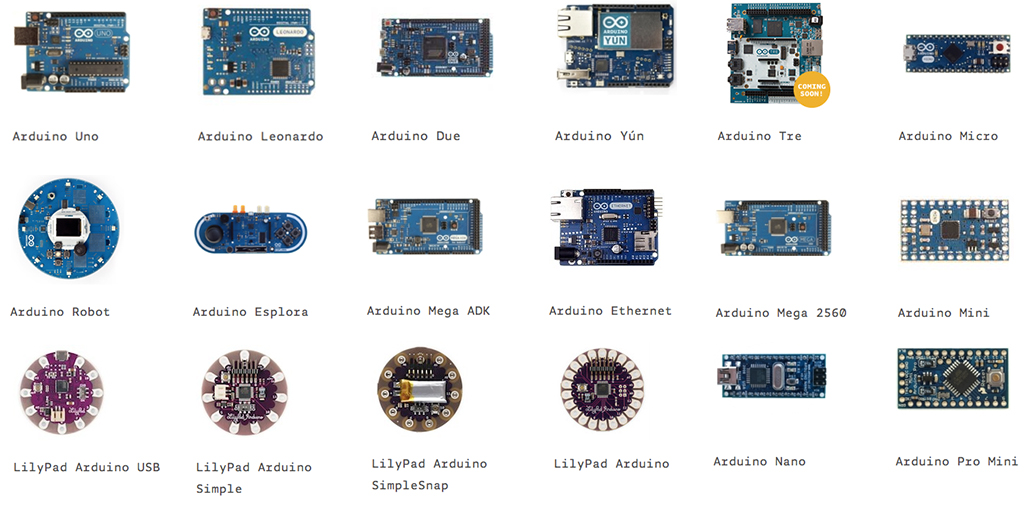
\includegraphics[width=0.9\linewidth]{ArduinoFamily}
	\caption[Arduino család néhány fajtája]{Arduino család néhány fajtája}
	\label{fig-arduinofamily}
\end{figure}
\subsection{Arduino Nano}
Elsősorban UNO-val\cite{arduinouno} terveztem elkészíteni ezt a projektet, de helyszűkében kénytelen voltam egy kisebb mikrokontroller után kutatni. Ekkor esett a választásom az Arduino Nano-ra\cite{arduinonano}. Az Arduino Nano az Arduino UNO kompaktabb változata, mely ugyanazt az ATmega328 mikrovezérlőt használja, így teljesítményében és képességeiben nagyon hasonló az UNO-hoz. A mikrovezérlő tartalmaz:
\begin{itemize}
	\item Processzort
	\item Memóriát
	\item Perifériákat:
	\begin{itemize}
		\item Időzítő áramkörök
		\item Analóg és digitális be- és kimenetek
		\item Kommunikációs interfészek (UART, SPI, I2C) és egyéb funkciók
	\end{itemize}
\end{itemize}

\begin{figure}[th!]
	\centering
	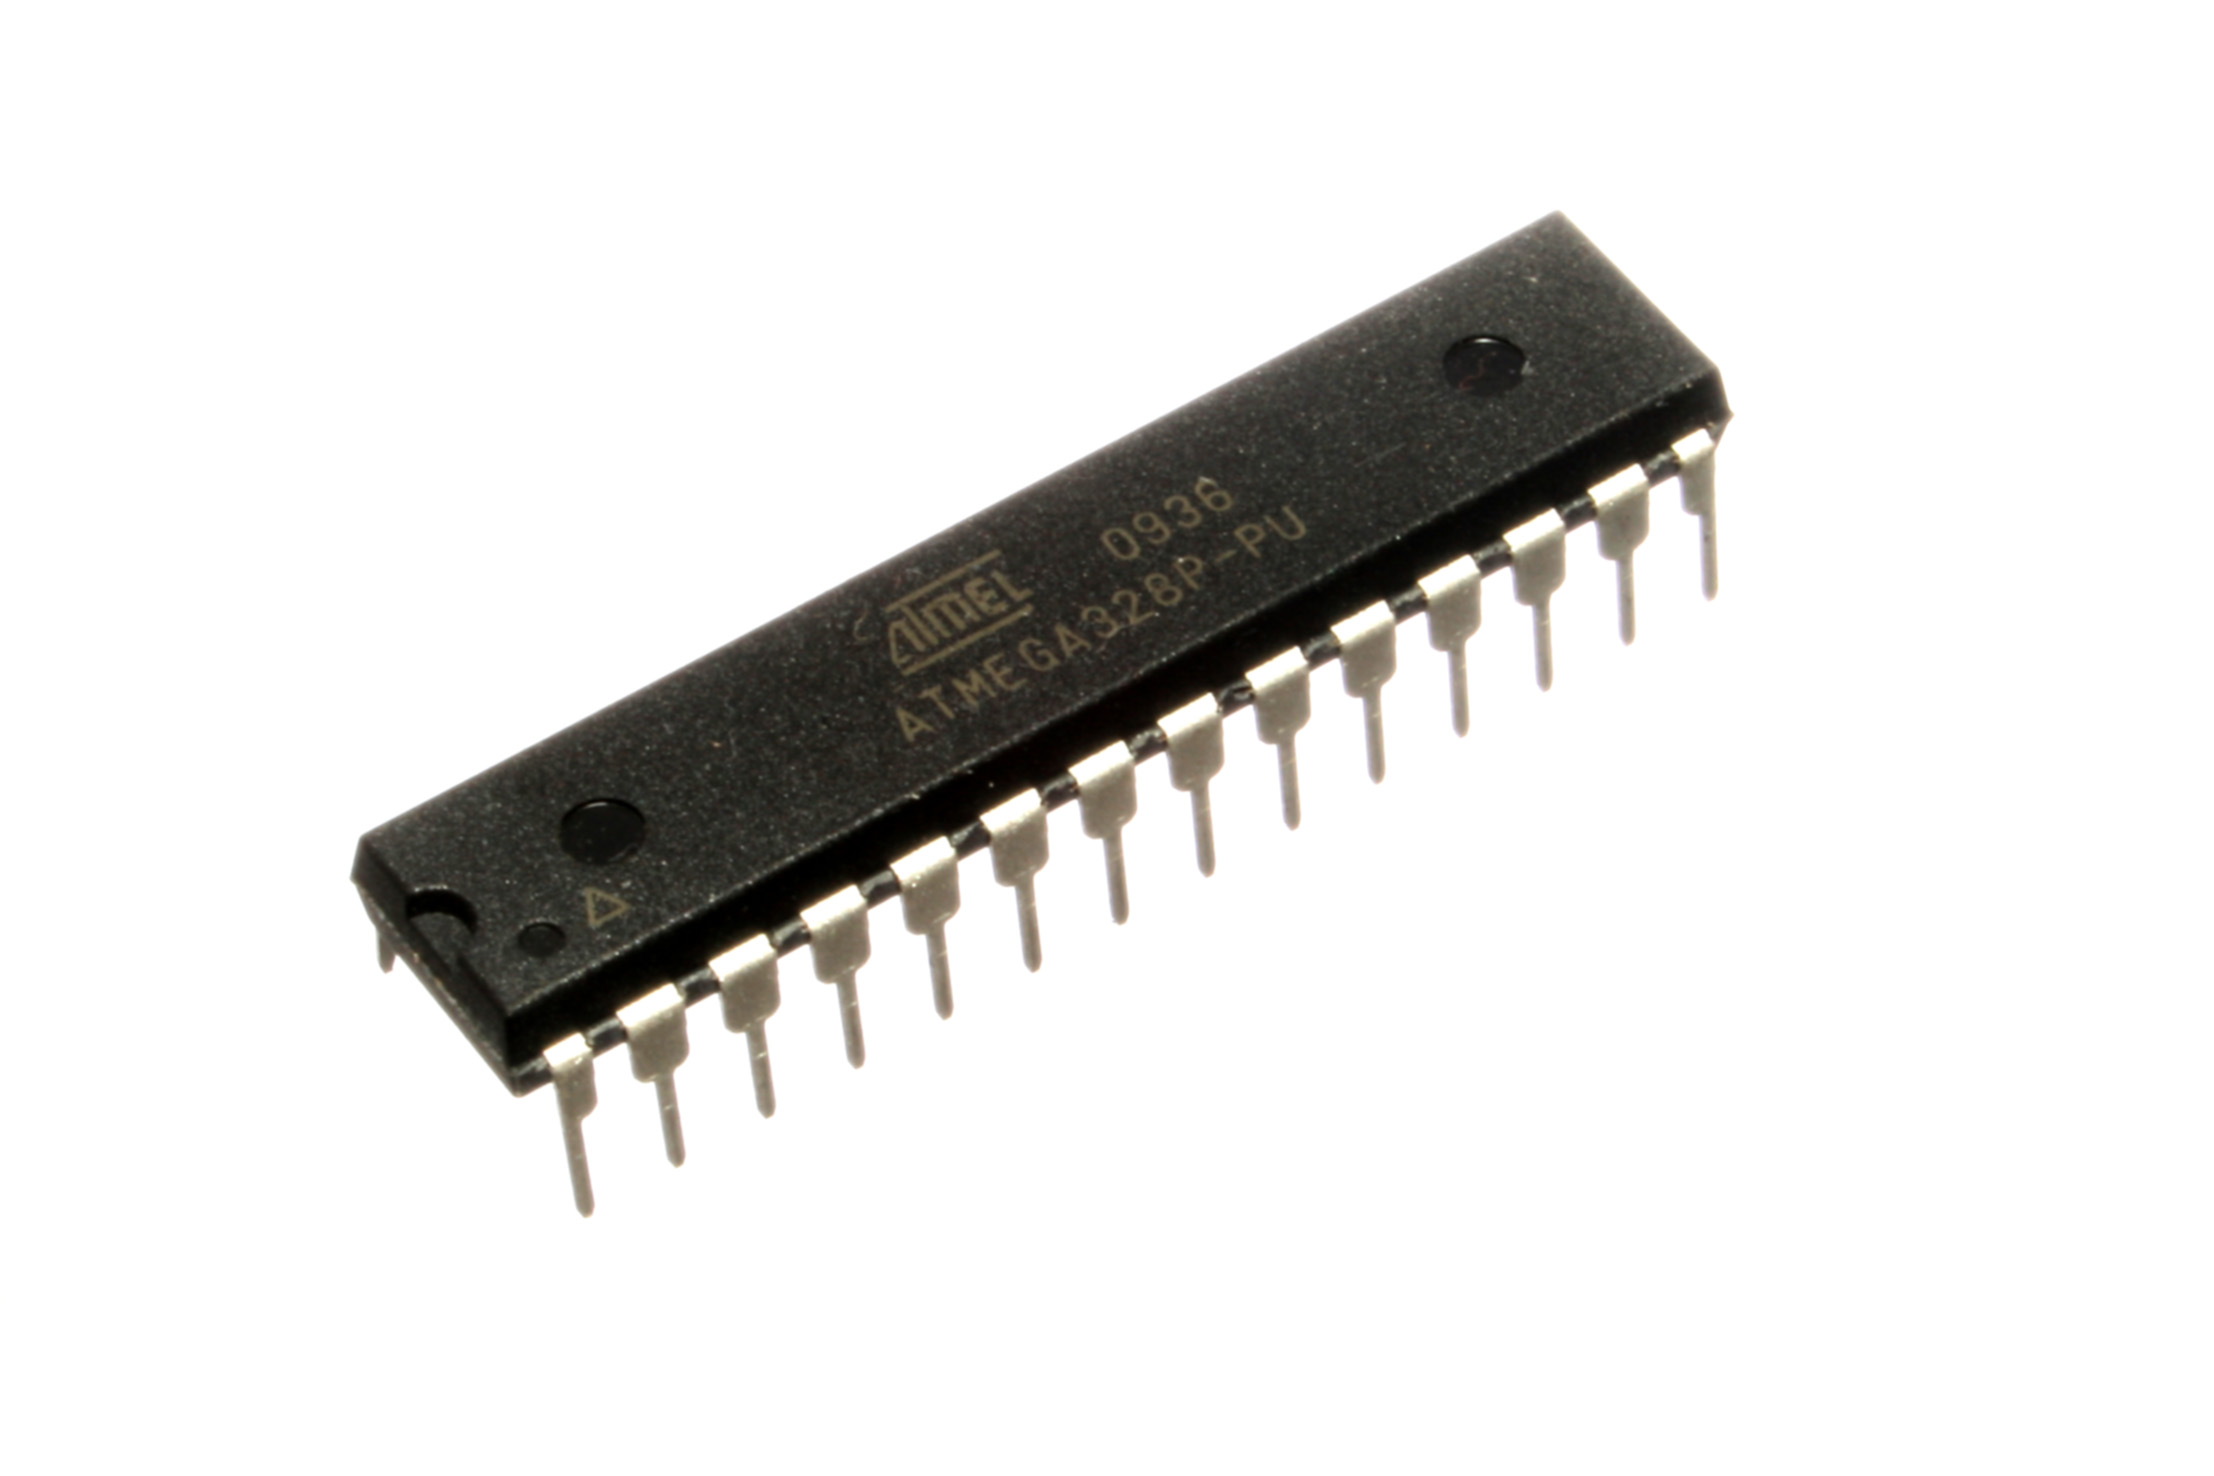
\includegraphics[width=0.4\linewidth]{ATMEGA328P-PU}
	\caption[ATmega328P]{ATmega328P mikrovezérlő}
	\label{fig:atmega328p-pu}
\end{figure}

Ezek segítségével tudunk szenzorjeleket mérni, nyomógombok vagy más beviteli eszközök állapotát beolvasni. A Nano áramköri lap szerepe az, hogy a mikrovezérlő lábait kivezesse. Így kényelmesebben és egyszerűbben rá tudjuk kötni a különböző eszközöket, amiket vezérelni szeretnénk, vagy értékeket beolvasni róluk. 

A mikrokontrollereken általában nem fut operációs rendszer, ezért minden erőforrást a feladatra összpontosít és egy garantált maximális idő alatt képes végre hajtani a feladatokat. 

Ahhoz, hogy külső eszközöket és áramköröket rátudjunk csatlakoztatni, ismernünk kell a Nano lábkiosztását, amikre a kódból tudunk hivatkozni és vezérelni őket, áramköri lapon fel van tüntetve, hogy melyik lábat melyik számmal érjük el.  A Nano-n 14 digitális ki- és bemenet található (D0–D13), valamint 8 analóg bemenet (A0–A7), melyek közül az A0–A5 lábak digitális bemenetként és kimenetként is használhatók. A Nano-n található továbbá fix 3.3,V és 5,V-os kimeneti feszültségű láb is. Ez a lábkiosztás látható \aref{fig:arduino-nano-pinout}. számű ábrán.

\begin{figure}[th!]
	\centering
	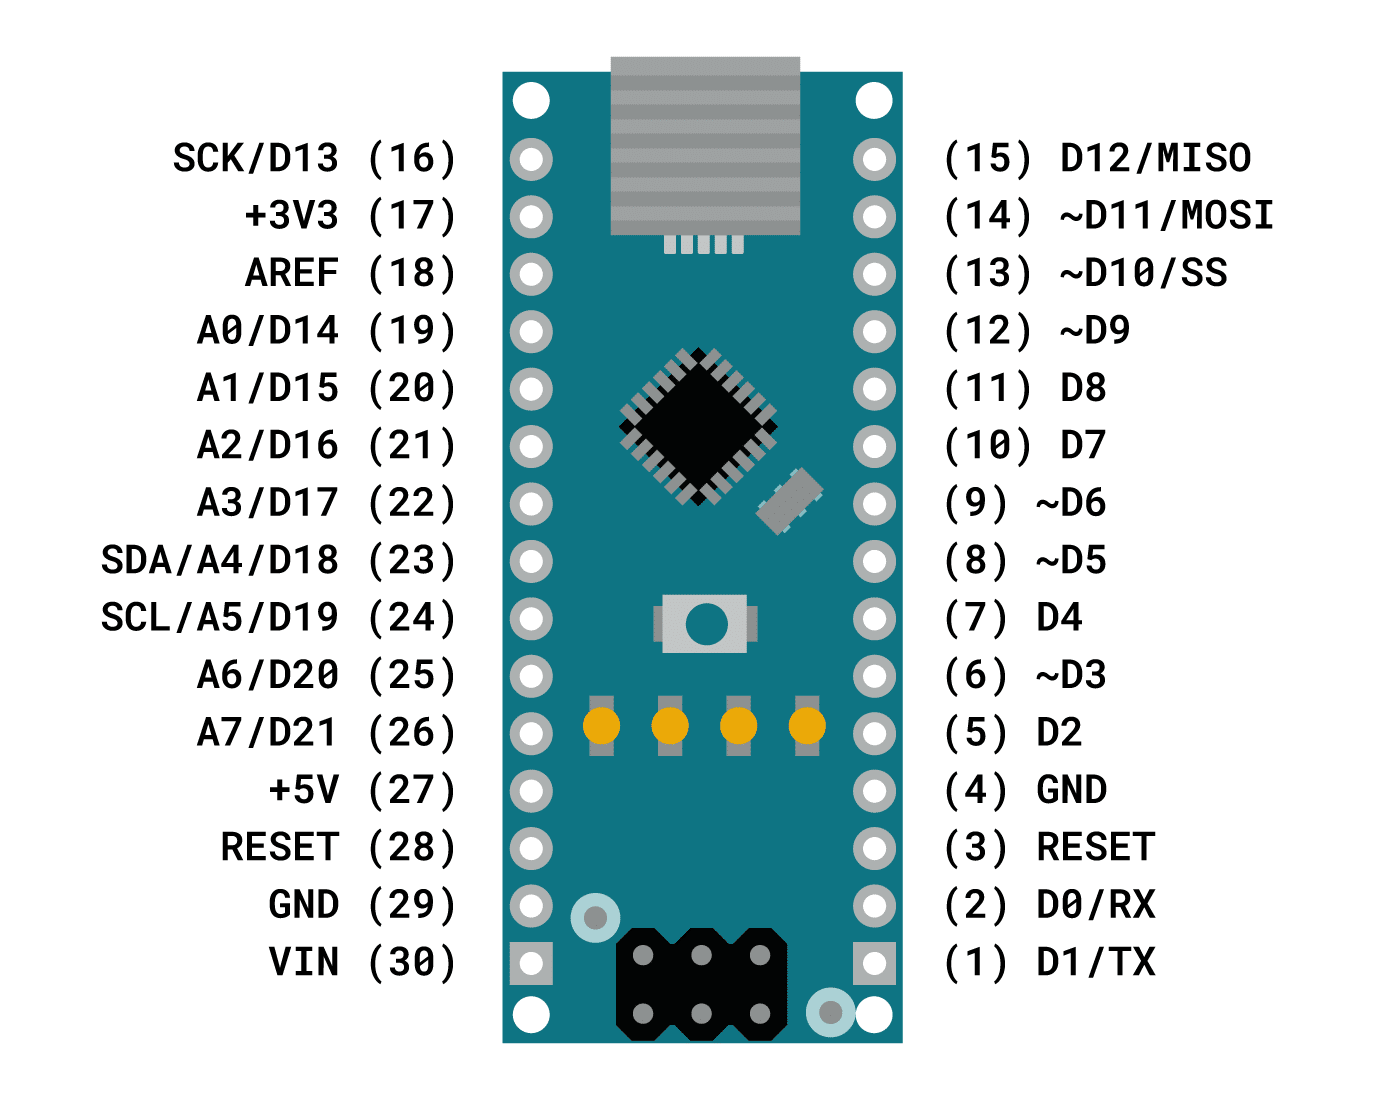
\includegraphics[width=0.7\linewidth]{arduino-nano-pinout}
	\caption[Nano felépítés]{Arduino Nano lábkiosztása}
	\label{fig:arduino-nano-pinout}
\end{figure}

\subsection{Miért választottam az Arduino Nano-t?}
Szakdolgozatom során az Arduino Nano-t választottam, mivel több olyan előnye van, amelyek különösen fontosak a projektem szempontjából:

\begin{itemize}
	\item \textbf{1. Kompakt méret.} A Nano mérete kisebb, mint az UNO-é, így ideális választás volt, mivel helyszűkében voltam.
	\item \textbf{2. Egyszerű használat és támogatottság.} Az Arduino Nano széles körben elterjedt mikrokontroller, amelyhez könnyen elérhetőek könyvtárak és példakódok, ezzel egyszerűsítve a fejlesztést.
	\item \textbf{3. Megfelelő teljesítmény és elegendő számú I/O port.} A Nano szintén ATmega328 mikrovezérlőt használ, amely tökéletesen megfelel az ADNS-9800 szenzor kezelésére, a szenzor mozgatására, valamint az adatok továbbítására.
	\item \textbf{4. Megbízhatóság és stabilitás.} A stabil működés létfontosságú, mivel a projektem dokumentumok folyamatos szkennelését, adatgyűjtést és adatátvitelt igényel hosszabb ideig.
	\item \textbf{5. Költséghatékonyság.} Az Arduino Nano az egyik legkedvezőbb árú fejlesztőeszköz, amely tökéletesen kielégíti a projekt követelményeit.
	\item \textbf{6. Egyszerű programozhatóság és csatlakoztatás.} Az Arduino Nano könnyen programozható az Arduino IDE használatával, programokat egyszerűen USB-n keresztül tölthetünk fel rá.
\end{itemize}
\subsection{Az Arduino alkalmazási területei}
\begin{itemize}
	\item \textbf{Kezdő projektekhez.} Az Arduino Board-ok tökéletesek a kezdők számára akik az elektronikát és az informatikát szeretnék ötvözni. A fejlesztő környezetet egyszerű kezelni, valamint a könyvtárak és a példa kódok is nagyon sokat segítenek azoknak az embereknek akik elkezdenek érdeklődni az ilyen dolgok iránt.
	\item \textbf{Oktatási platform.} Könnyen kezelhetősége miatt szokták alkalmazni, hogy ezekkel az eszközökkel tanítsák meg az elektronika és az informatika működését.
	\item \textbf{Robotikában.} A nagy vállalatok vezetői is felfedezték ezt a technológiát, és gyakran Arduino Board-okat használnak a robotok megvalósításához és vezérléséhez.
	\item \textbf{Zene és művészet.} Az Arduino Board-okat szokták egyszerű hangszerek létrehozására is alkalmazni, vagy már meglévő hangszerekbe beépíteni elektronikus alkatrészként.
	\item \textbf{IoT - Internet of Things.} Legtöbb esetben okos otthon rendszerekbe szokták beépíteni, mert sok szenzort rá tudunk csatlakoztatni amikkel könnyen vezérelhetjük a saját otthonunkat. 
	\item \textbf{Viselhető eszközök. (Wearables)} Kompakt méretük miatt könnyen beépíthetőek ruhákba, akár ékszerekbe vagy más hordozható eszközökbe. Amelyekkel mozgásokra reagálhatunk mérhetünk testhőmérsékletet és még sok mást.
\end{itemize}
\section{Visual Studio}
A projekt szoftveres részét Visual Studio\cite{visual-studio} fejlesztői környezettel készítettem el, mert ez áll hozzám a legközelebb. Itt valósítottam meg az interpolációt a kép minőségvesztés nélküli növelését. Valamint a program irányító felületét is itt programoztam le. 
\section{Github}
A verziókövetéshez a Githubot\cite{github} használtam azon belül is a Github Desktop-ot, mellyel könnyen tudtam több platformon is dolgozni a projekten, valamint ha valamit elrontottam könnyen vissza tudtam állítani a projektet egy korábbi verzióra.
\chapter{Hardveres megvalósítás}
\section{ADNS-9800 szenzor}
Az általam készített szkennernek a lelke a kicsi és olcsó ADNS-9800\cite{adns9800} lézeres optikai érzékelő. Az eredeti felhasználási módja ennek az eszköznek az volt, hogy egerek mozgását kövessék. Ennek a szenzornak az a különlegessége, és azért volt megfelelő számomra, mivel úgy követi a mozgást, hogy folyamatosan képeket készít. Ezáltal fel tudtam használni a projektembe, mint egy kis kamerát, valamint gyors képfeldolgozási képességgel rendelkezik, ezért alkalmas dokumentumok beolvasására. 
\subsection{Működése}
 A szenzor működésének alapja a LaserStream technológia, amely során egy beépített lézer folyamatosan megvilágítja a felületet. A lencse ezt követően készít egy képet és a beépített digitális jelfeldolgozó (DSP) valós időben matematikai úton kiszámítja a felület elmozdulásának irányát és mértékét. Ez a megoldás lehetővé teszi a nagyon pontos mozgásérzékelést, hiszen a szenzor akár 8200 cpi (counts per inch) felbontással is képes mérni a mozgást.
\begin{figure}[th!]
	\centering
	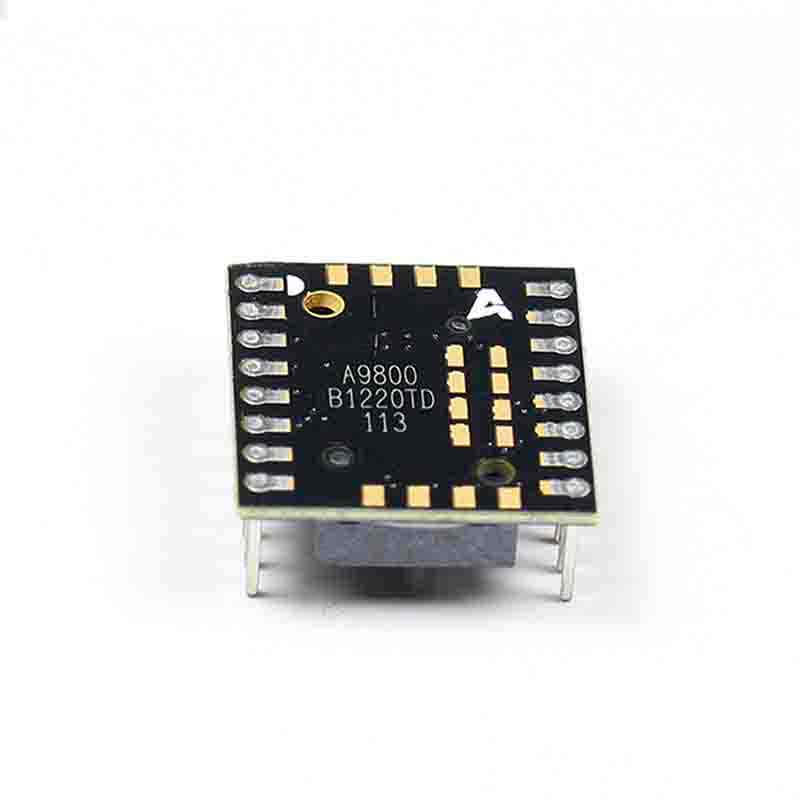
\includegraphics[width=0.35\linewidth]{ADNS9800base}
	\caption[ADNS9800]{ADNS-9800 szenzor}
	\label{fig:adns9800base}
\end{figure}

Az általam választott szenzor már nyáklappal volt ellátva, ami nagymértékben egyszerűsítette a beépítési folyamatot. 

\begin{figure}[th!]
	\centering
	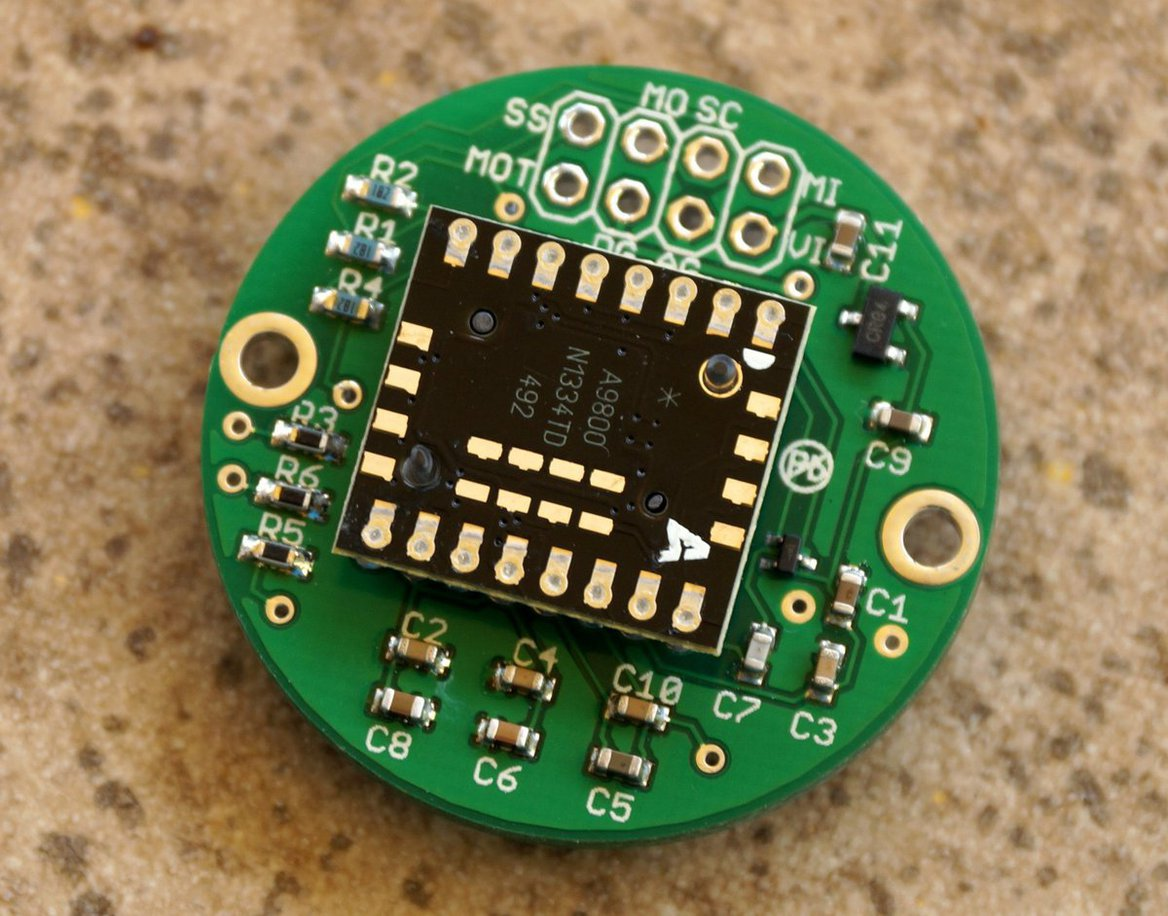
\includegraphics[width=0.3\linewidth]{ADNS9800}
	\caption[ADNS9800]{ADNS-9800 szenzor nyák lapra szerelve}
	\label{fig:adns9800}
\end{figure}

Csak egy problémám volt, hogy a nyáklappal szerelt verzió 3.3\,V-os logikai szinttel működött viszont az Arduino Nano 5\,V-os jeleket használ. Így be kellett szereznem egy két irányú logikai szintillesztő\cite{szintilleszto} modult ami átalakította a 3,3\,V-os  jelet 5\,V-ossá. Ehhez a projekthez egy 8 csatornás logikai szintillesztő modult használtam.

\begin{figure}[th!]
	\centering
	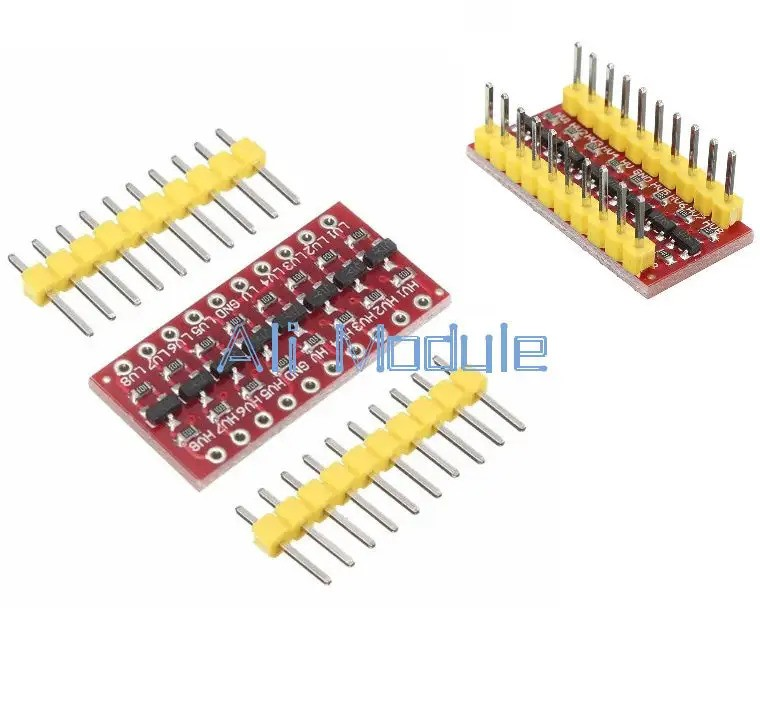
\includegraphics[width=0.4\linewidth]{szintilleszto}
	\caption[Logikai szintillesztő]{Két irányú logikai szintillesztő}
	\label{fig:szintilleszto}
\end{figure}
\subsection{Adatok beolvasása}
Az adatok beolvasása közben a szenzor egy sorokból és egy oszlopokból álló képkockát készít, amely egy 30\,x\,30-as pixel rács. Ezáltal egy dokumentum szkennelése lehet akár több ezer képkocka is.
A működése a következő lépésekből áll:
\begin{enumerate}
	\item \textbf{Feltöltjük a firmware-t a szenzorra.} Erre azért van szükség, mert enélkül a szenzor csak egy hardveres érzékelő, amely a lézerrel megvilágított felületről képeket készít. Ahhoz, hogy ezt az információt feldolgozza és továbbítsa szüksége van egy vezérlőprogramra, azaz firmware-re. Ezt a firmware-t minden bekapcsolás után fel kell tölteni, mert a szenzornak nincs állandó memóriája. A regiszterek megfelelő beállítása után a firmwaret soronként továbbítja  az SPI buszon keresztül a szenzornak. Ebben a metódusban fontos az időzítés, hogy a szenzor helyesen értelmezze az adatokat.
	\begin{lstlisting}[language=Arduino,label=upload-firmware-code]
		void adns_upload_firmware(){
			adns_write_reg(REG_Configuration_IV, 0x02);	
			adns_write_reg(REG_SROM_Enable, 0xd); 
			delay(10); 
			adns_write_reg(REG_SROM_Enable, 0x8); 
			adns_com_begin();
			SPI.transfer(REG_SROM_Load_Burst | 0x80); 
			delayMicroseconds(15);
			unsigned char c;
			for(int i = 0; i < firmware_length; i++){ 
				c = (unsigned char)pgm_read_byte(firmware_data + i);
				SPI.transfer(c);
				delayMicroseconds(15); 
			}
			adns_com_end();
		}
	\end{lstlisting}
	%%talán bele lehetne vinni a winforms-os elindítást
	\item Majd a \textbf{sendFrame()} metódust meghívva készítünk egy képet a szenzorral. Amit egy nagy sebességű, full--duplex kommunikációs protokollal (Serial Peripheral Interface~--~SPI) kiolvasunk és eltároljuk, ahol a kommunikáció egy órajel vezérelt mechanizmussal működik. 
	\begin{lstlisting}[language=Arduino,label=sendFrame]
		void sendFrame() {
			adns_write_reg(REG_Power_Up_Reset, 0x5A);
			delay(50);
			adns_write_reg(REG_LASER_CTRL0, 0x00);
			adns_write_reg(REG_Frame_Capture,0x93);
			delayMicroseconds(120); 
			adns_write_reg(REG_Frame_Capture,0xc5);
			delayMicroseconds(120); 
			delay(1); 
			adns_com_begin(); 
			delayMicroseconds(100); 
			byte readys = 0;
			while(readys == 0){
				SPI.transfer(REG_Motion & 0x7f);
				delayMicroseconds(100); 
				readys = SPI.transfer(0); 
				readys = readys & 1;
				delayMicroseconds(20);
			}
			SPI.transfer(REG_Pixel_Burst & 0x7f); 
			delayMicroseconds(100); 
			Serial.print("FRAME:");
			for (int i = 0;i<900;i++){
				byte pixelValue = SPI.transfer(0);  
				Serial.print(pixelValue);
				Serial.print(" ");
			}
			delayMicroseconds(15); 
			adns_com_end();  
			delayMicroseconds(5); 
			Serial.println();
		}
	\end{lstlisting}
	A metódus működése:
	\begin{enumerate}[label=\arabic*.]
		\item \textbf{Szenzornak kiadjuk, hogy készítsen egy képet.} Ekkor bele írjuk a megfelelő értéket a REG\_Frame\_Capture regiszterbe. A szenzor ekkor egy 30\,x\,30 pixeles képkockát olvas be.
		\item \textbf{Várunk amíg a szenzor elkészíti a képet.} Az Arduino egy ciklusban folyamatosan ellenőrzi a szenzor állapotát ezért amíg a szenzor nem jelez, nem olvassuk ki az értéket.
		\item \textbf{A szenzor továbbítja a képkockát.} A Pixel Burst regiszteren keresztül történik a képkocka eljuttatása a szenzortól az Arduino-ig SPI kapcsolattal. Az SPI kapcsolat négy vezetéken keresztül történik:
		\begin{itemize}
			\item \textbf{MOSI }(Master Out, Slave In): Az adatok a mikrokontroller felől a szenzor felé mennek.
			\item \textbf{MISO }(Master In, Slave Out): Az adatok a szenzor felől mennek az Arduino felé.
			\item \textbf{SCLK }(Serial Clock): Az órajel, amelyet az Arduino generál.
			\item \textbf{CS }(Chip Select): Az adott szenzort választja ki a kommunikációhoz.
		\end{itemize}
		\item \textbf{Az Arduino továbbítja az adatokat a számítógépre.} Az adatok soros kommunikáción keresztül kerülnek a számítógépre ahol az feldolgozza ezeket. Minden képkocka ''FRAME:'' előtaggal kezdődik, amit a szenzor által olvasott fényintenzitás értékek követnek. Egy példa frame sor:
		
		\verb|FRAME: 124 128 130 122 120 119 118 117 116 ...|
	\end{enumerate}
\end{enumerate}
\subsection{Szenzor mozgása}

A szenzort két motor mozgatja az egyik vízszintesen a másik pedig függőlegesen. A projekthez egy bipoláris valamint egy unipoláris léptetőmotort\cite{motorvezerlok} használtam. Mivel egy meglévő szkennerbe építettem bele az egész elektronikát, ezért a függőleges tengely mozgatására szolgáló bipoláris léptetőmotor már adott volt. Viszont a szenzor nagyon kis képet készít ezért finom mozgásokra volt szükségem, ebben segítséget nyújtottak a már előre beépített fogaskerekek, amik áttétként funkcionálnak. Ezáltal a motor egy lépése jelentősen kisebb elmozdulás volt fizikailag, így jól tudtam pozicionálni. A motort egy L298N\cite{l298n} motorvezérlőn keresztül irányítottam.
\begin{figure}[th!]
	\centering
	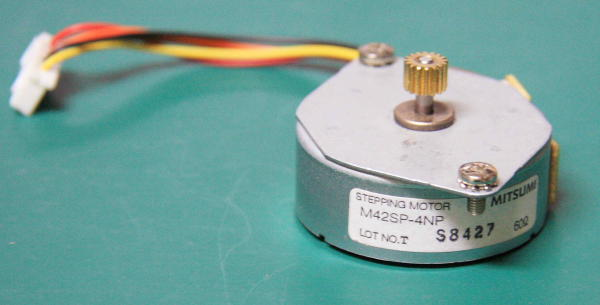
\includegraphics[width=0.4\linewidth]{MITSUMI-Stepping-Motor-M42SP-4NP}
	\caption[Mitsumi]{\footnotesize {MITSUMI M42SP-4NP bipoláris motor a függőleges mozgáshoz}}
	\label{fig:mitsumi-stepping-motor-m42sp-4np}
\end{figure}

Mindkét motornál half-step vezérlési módot használtam, hogy még finomabb és pontosabb mozgást tudjak végezni velük. Ennek az a lényege, hogy a motor kétszer annyi lépésben teszi meg ugyanazt a fordulatot. Ez úgy lehetséges, hogy a négy tekercs közül először egy tekercs kap áramot, majd az első és a második egyszerre, majd csak a második, így a lépés szám a duplájára nő a szögelfordulás pedig a felére csökken.

\begin{figure}[th!]
	\centering
	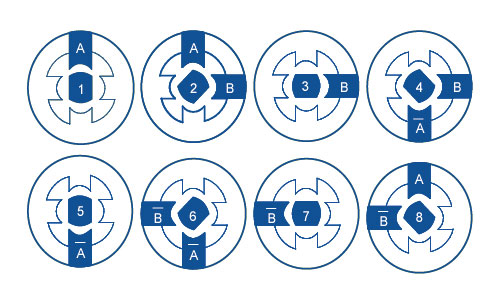
\includegraphics[width=0.5\linewidth]{stepper-motors-half-step}
	\caption[Half Step vezérlés]{Half Step vezérlés működése}
	\label{fig:stepper-motors-half-step}
\end{figure}


A vízszintes mozgáshoz beépítettem egy unipoláris léptetőmotort, amely egy ULN2003 motorvezérlő modullal működik, amit nagyon gyakran használnak ilyen kis apró finom mozgásokhoz, amire nekem is szükségem volt. Mivel ez a motor úgy van felépítve, hogy alapból áttétek vannak benne ezért azzal itt sem kellett foglalkoznom. A motorok egy egy bordás szíjas sínen mozognak, ezáltal a mozgás stabil lesz és csúszásmentes. Mindkettő végén van egy végállás kapcsoló, ha a vízszintes sor a végére ér ezt aktiválja és lentebb megy egy sort, valamint vissza megy a sor elejére a szenzor. Ekkor küld az Arduino egy ''NEW\_ROW'' kulcsszót a Serial porton a számítógép felé, ezzel jelezve a feldolgozó szoftvernek, hogy új sor következik az olvasásban. Ha pedig a függőleges végálláskapcsoló válik aktívvá akkor pedig az ''END'' kulcsszót küldi el a számítógép felé, jelezve, hogy vége a dokumentumnak és vissza tér a kezdeti állásba.

\begin{figure}[th!]
	\centering
	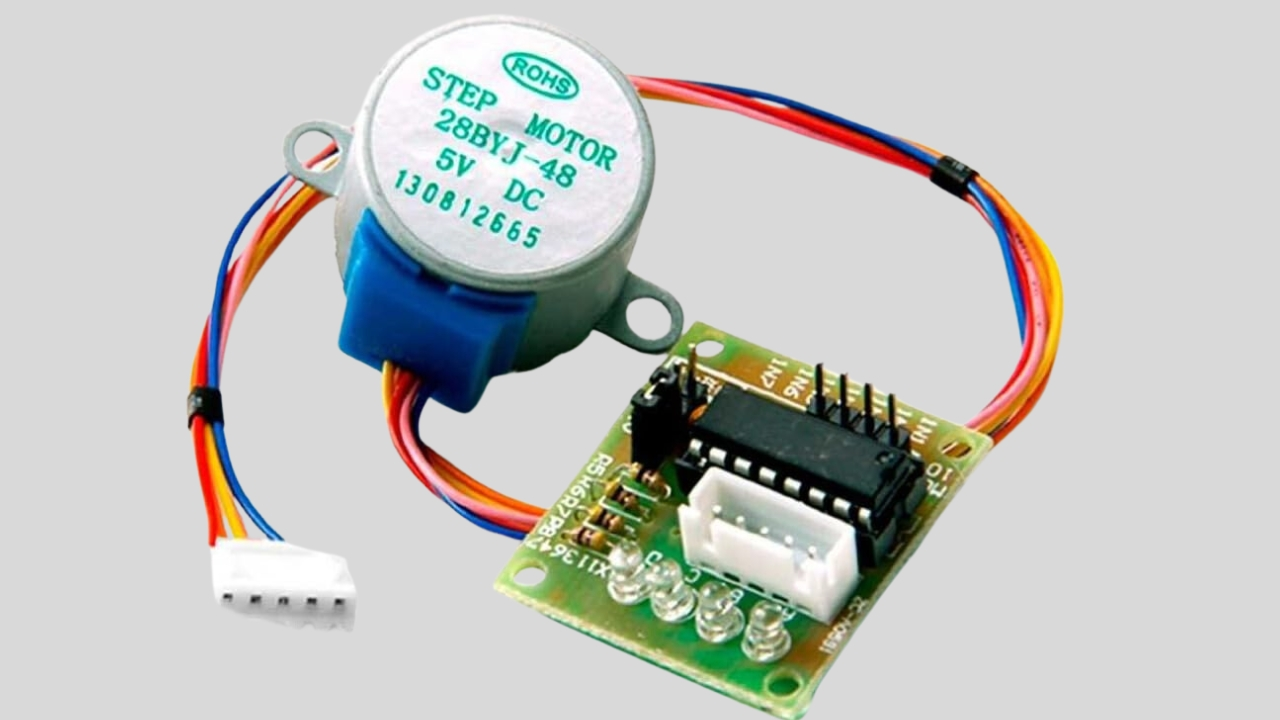
\includegraphics[width=0.5\linewidth]{28BYJ-48-modul-ULN2003}
	\caption[Unipoláris léptetőmotor]{Unipoláris léptetőmotor a vízszintes mozgáshoz}
	\label{fig:28byj-48-modul-uln2003}
\end{figure}

A szenzor mozgatásához még szükségem volt két darab Infravörös szenzorra amik a segítségével a szenzor kezdőállását tudtam meghatározni. Ez egy egyszerű kis szenzor ami infravörös fényt bocsát ki az egyik oldalt és a másik oldalt van egy infravörös vevő egység és ha megszakad a jel, például valamit közé helyezünk, akkor ad magas jelet a szenzor. 
 \begin{figure}[th!]
 	\centering
 	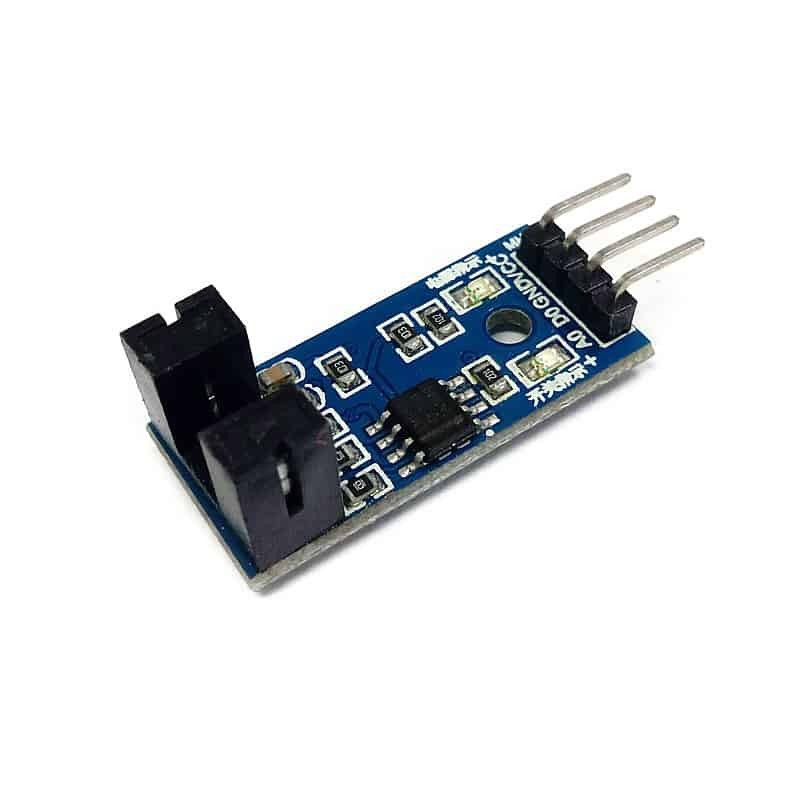
\includegraphics[width=0.4\linewidth]{MH-Infrared-Speed-Sensor-Module}
 	\caption[Infravörös kapu]{Infravörös kapu}
 	\label{fig:mh-infrared-speed-sensor-module}
 \end{figure}

\section{Hardveres bekötés}
A bekötési rajzon narancssárgával színezett elemek a motorvezérlők, pontosan az L298N és az ULN2003AN. A kék színű elem a szintillesztő és a zöld pedig az ADNS-9800 szenzor. Valamint van még két motor, két infravörös érzékelő és az Arduino Nano.
\begin{figure}[th!]
	\centering
	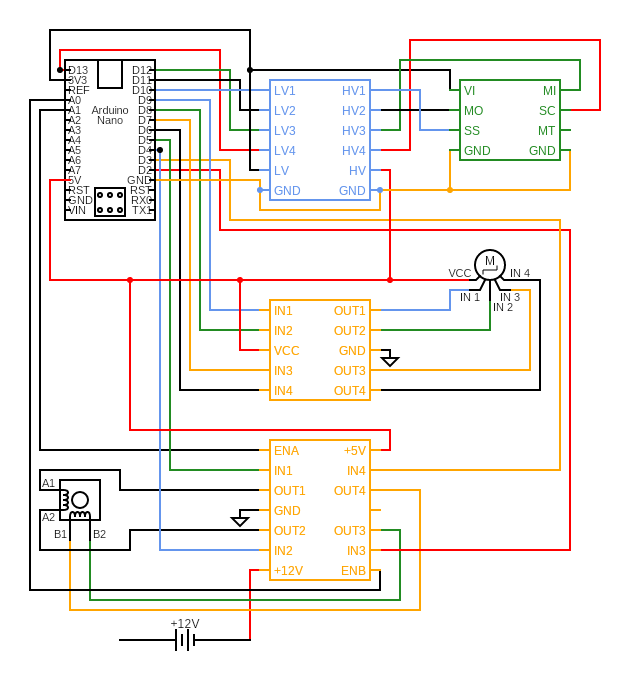
\includegraphics[width=1\linewidth]{circuit}
	\caption[Hardveres bekötés]{Hardveres bekötés}
	\label{fig:circuit}
\end{figure}
\chapter{Szoftveres megvalósítás}

%%\section{Felhasznált algoritmusok/metódusok}
%%\section{Beolvasott értékek tárolása 2 dimenzós mátrixban}
%%adatszeerkezet amiben a beolvasott képet tároljuk
%%\section{Bikubik interpoláció}
%%\subsection{Működése}
%%Működésének alapjai, Matematikai leírása
%%\section{Mátrix átalakítása képpé}

\section{Az alap változók}
A feldolgozó szoftver Serial porton kapja meg az adatokat az Arduino-tól. Van két darab konstans értékem az egyik a beérkező képkocka szélessége a másik pedig a magassága, mivel a beérkező képkocka 30\,x\,30 pixel ezért ez a két érték 30. Van egy buffer-em ahol a Serial porton beérkező adatokat tárolom, erre azért van szükség mert nem biztos, hogy egy sor át tud jönni egyszerre. Valamint van egy Bicubic osztály példányom amivel a Bikubikus interpolációt végzem. Végül van egy \emph{row} és egy \emph{column} változóm ami annak segítségére szolgál, hogy összerakjam a képkockákat egy nagy dokumentummá. Ezt a nagy dokumentumot tartalmazza a \emph{listGrid} nevű változó, ami egy lista amiben listák vannak amiben egész típusú tömbök vannak. 
\begin{lstlisting}[language=CSharp]
private SerialPort serialPort;
private const int FrameWidth = 30; 
private const int FrameHeight = 30; 
private StringBuilder dataBuffer = new StringBuilder(); 
private const int scale = 2;
private Bicubic resizer = new Bicubic(FrameWidth, FrameHeight, scale);

int row = 0;
int column = 0;

private List<List<int[]>> listGrid = new List<List<int[]>>();
\end{lstlisting}

\section{Inicializáló metódusok}
Van egy soros portot beállító metódus. Aminek segítségével megnyitom a soros portot és beállítom a megfelelő BaudRate-t. Jelen esetben 115200 bit/másodperc. Hozzárendelem a serialPort változó DataReceived eseményéhez a saját metódusomat, ami azt jelenti, hogy amikor érkezik adat a soros porton akkor meghívja azt a metódust. Ezután megnyitom a soros portot, hogy tudjam olvasni az adatokat róla, és írok egy ''reset'' kulcsszót az Arduino felé ezen a porton keresztül, hogy alaphelyzetbe tegyem a szenzort.
\begin{lstlisting}[language=CSharp]
	private void InitializeSerialPort()
	{
		serialPort = new SerialPort("COM3", 115200);
		serialPort.DataReceived += DataReceived;
		serialPort.Open();
		serialPort.Write("reset");
	}
\end{lstlisting}

\section{Bejövő adatot feldolgozó metódus}
A bejövő adatokat egy külön metódus kezeli. A metódus elején megnézem, hogy a beérkezett data üres-e, ha igen akkor jelzem a hibát és kilépek. Viszont ha van adat akkor azt hozzáadom a dataBufferhez ami tárolja az eddig beérkezett adatokat. Átalakítom a jelenlegi dataBuffert String-é, hogy könnyebb legyen vele dolgozni. Végül deklarálok egy változót amiben az aktuális sor végén lévő új sor karakter pozícióját tárolom.
\begin{lstlisting}[language=CSharp, basicstyle=\small]
private void ProcessSerialData(string data)
{
	if (string.IsNullOrEmpty(data))
	{
		MessageBox.Show("A beérkezett adat üres", "Hiba", MessageBoxButtons.OK, MessageBoxIcon.Error);
		return;
	}
	dataBuffer.Append(data); 
	string bufferString = dataBuffer.ToString();
	int newlineIndex;
\end{lstlisting}
Az adatok feldolgozását egy while ciklus végzi ami addig megy amíg a bufferstring tartalmaz új sor jelet, eközben a ciklus minden iterációjában kimentem a jelenlegi indexét az új sor jelnek. Ezen belül kinyerem az első teljes sort a bufferből és levágom a felesleges szóközöket. Eltávolítom ezt a teljes sort a dataBufferből. Frissítem a bufferstring változót is, hogy csak a még fel nem dolgozott rész maradjon. Mivel WinForms-al dolgozok ezért szükségem van az InvokeRequired feltételre, amivel megvizsgálom, hogy az adott hívás másik szálról történik-e, ha a hívás a főszálon történik akkor csak egyszerűen hozzáadom a listboxhoz a beérkezett adatot, ha nem akkor az Invoke metódussal hozzá adom a főszálon.
\begin{lstlisting}[language=CSharp]
	while ((newlineIndex=bufferString.IndexOf("\n"))!= -1)
	{
		string fullLine = bufferString.Substring(0, newlineIndex).Trim(); 
		dataBuffer.Remove(0, newlineIndex + 1);
		bufferString = bufferString.Substring(newlineIndex + 1);
		if (this.InvokeRequired)
		{
			this.Invoke(new Action(() => listBox1.Items.Add("Beérkező sor: "+fullLine)));
		}
		else
		{
			listBox1.Items.Add("Beérkező sor: " + fullLine);
		}
\end{lstlisting}
Ha a jelenlegi beérkezett sor úgy kezdődik, hogy ''FRAME'' akkor levágom az elejéről a ''FRAME'' szót és a maradék adatot kimentem egy szöveg típusú tömbbe. Leellenőrzöm, hogy ennek a tömbnek megegyezik-e a hossza az általam előírttal. Tehát az alap \emph{FrameWidth} és \emph{FrameHeight} szorzatával ami 30\,x\,30, ha nem akkor hibát dobok. Az interpolációs osztály példányával meghívom erre a tömbre az interpoláló metódust, közben az összes elemet átalakítom egész típusú számmá és kimentem egy \emph{frameData} nevű egész típusú tömbbe. Ezután megjelenítem a már interpolált képet az alkalmazásban egy pictureBox segítségével. Valamint megvizsgálom, hogy a \emph{row} változónak az értéke nagyobb-e, mint a \emph{listGrid} hossza, amivel itt a sor kezelést oldom meg, ha igen akkor azt jelenti, hogy már egy új sorban vagyunk már ezért kell hozzá adnunk egy új tömbökből álló listát. Végül hozzáadjuk a jelenlegi sorhoz a tömböt. 
\begin{lstlisting}[language=CSharp]
		if (fullLine.StartsWith("FRAME:"))
		{
			string[] pixels = fullLine.Substring(6).Split(new[] { ' ' });
			if (pixels.Length == FrameWidth * FrameHeight)
			{
				int[] frameData = resizer.BicubicResize(Array.ConvertAll(pixels, int.Parse));
				DisplayFrame(frameData, FrameHeight * scale, FrameWidth * scale);
				if (row >= listGrid.Count)
				{
					listGrid.Add(new List<int[]>());
				}
				listGrid[row].Add(frameData);
			}
			else
			{
				if (this.InvokeRequired)
				{
					this.Invoke(new Action(() => listBox1.Items.Add("Hibás FRAME sor hossz: "+pixels.Length)));
				}
				else
				{
					listBox1.Items.Add("Hibás FRAME sor hossz: "+pixels.Length);
				}
			}
		}
\end{lstlisting}
Ha a ''NEW\_ROW'' kulcsszóval kezdődik a jelenlegi adat akkor csak simán növelem a sor indexet. Mivel ekkor jelet kapok az Arduino felől, hogy a szkennelés a következő sorban folytatódik tovább. Ha az ''END'' kulcsszó van a jelenlegi adatban akkor pedig befejeződött a szkennelés tehát leállítom a szenzort valamint elmentem a dokumentumot.
\begin{lstlisting}[language=CSharp]
		if (fullLine.StartsWith("NEW_ROW"))
		{
			row++;	
		}
		if (fullLine.StartsWith("END"))
		{
			serialPort.WriteLine("stop");
			SaveDoc();
		}
	}
}
\end{lstlisting}
\section{Kiegészítő metódusok}
Az egyik legfontosabb kiegészítő metódus a \textbf{matrixToBitmap} amiben egy képkockákból álló két dimenziós listát alakítok át egy nagy szürkeárnyalatos Bitmap\cite{bitmap.class} képpé. A célja a metódusnak, hogy a szenzor által beolvasott és interpolált képkockákat egy nagy képpé összeállítsam. A listGrid szerkezet egy két dimenziós lista amely úgy értelmezhető, hogy az első dimenzió (külső lista) a sorokat jelenti, a második dimenzió (belső lista) pedig az oszlopokat jelképezi. Végül minden int[\,] elem egy képkockát tartalmaz ahol a fényintenzitások sorban vannak felsorolva. 

Példa: listGrid[1][2] jelenti a második sor harmadik képkockáját.

Visszatérve a metódusra az egész metódus kezdődik egy ellenőrzéssel ahol megnézzük, hogy a \emph{listGrid} üres-e, ha igen akkor hibát dobunk.
\begin{lstlisting}[language=CSharp]
	  private Bitmap matrixToBitmap()
	 {
	 	if (listGrid.Count == 0 || listGrid[0].Count == 0 || listGrid[0][0] == null)
	 	{
	 		MessageBox.Show("A mátrix üres, nem lehet képet generálni.", "Hiba", MessageBoxButtons.OK, MessageBoxIcon.Error);
	 		return null;
	 	}
\end{lstlisting}
Meghatározzuk a képkockák szélességét és magasságát úgy, hogy megszorozzuk a nagyítási változóval az eredeti kép méreteit. Ezután meghatározzuk a teljes összeállított képek méretét.
\begin{lstlisting}[language=CSharp]
	 	int frameWidth = FrameWidth * scale;
	 	int frameHeight = FrameHeight * scale;
	 	int width = listGrid[0].Count * frameWidth;
	 	int height = listGrid.Count * frameHeight;
\end{lstlisting}
Az általános \textbf{SetPixel} metódus helyett én inkább a \textbf{LockBit} megoldást választottam, igaz, hogy az nem olyan egyszerű de a nagy képeknél viszont sokkal gyorsabb teljesítményt tudok elérni vele. Ennek az oka, hogy a memóriába írok közvetlenül a GDI hívások helyett.

Létrehozok egy Bitmap példányt 24 bites RGB formátumban, ami azt jelenti, hogy minden képpont 3 bájtot foglal el. A Rectangle osztállyal meghatározom a Bitmap teljes tartományát. A Bitmap \textbf{LockBits} metódusának átadom az előzőleg meghatározott rectangle-t, az ImageLockMode-ot amivel úgy zárom le a Bitmap-et, hogy csak írni tudjam,olvasni ne. Valamint átadom neki a Bitmap formátumát is, és vissza kapok egy BitmapData értéket ami tartalmazza ennek a zárolásnak az információit. Ebből kinyerve megkapom a stride-ot ami egy fontos információ, mivel ez mutatja meg, hogy a Bitmap memóriájában egy-egy sor hány bite hosszú. Ez nem feltétlenül egyezik meg a képpontok számának és a fényintenzitásnak megfelelő mérettel, mert a rendszer minden sort 4 bite-ra igazít a gyorsabb memóriakezelés miatt. Tehát ezzel fogom kiszámolni, hogy egy adott képpont hol helyezkedik el.
\begin{lstlisting}[language=CSharp]	 	
	 	Bitmap bmp = new Bitmap(width, height, PixelFormat.Format24bppRgb);
	 	Rectangle rect = new Rectangle(0, 0, width, height);
	 	BitmapData bmpData = bmp.LockBits(rect, ImageLockMode.WriteOnly, bmp.PixelFormat);	 	
	 	int stride = bmpData.Stride;
\end{lstlisting}
Végig megyek a \emph{listGrid}-en ami ugye a teljes nagy kép és ezen belül végig megyek a képkockákon is és minden egyes pixelt közvetlenül átmásolok egy byte tömbbe. Itt alkalmaztam egy kis kontraszt javítást is mert a szenzor képe nem a legszebb de így sokkal jobban néz ki. A stride segítségével kiszámolom, hogy az adott pozíció hányadik byte-nál kezdődik a memóriában.
\begin{lstlisting}[language=CSharp]	
		byte[] bytes = new byte[stride * height];
	 	for (int row = 0; row < listGrid.Count; row++)
	 	{
	 		for (int col = 0; col < listGrid[row].Count; col++)
	 		{
	 			int[] frameData = listGrid[row][col];
	 		
	 			int startX = col * frameWidth;
	 			int startY = row * frameHeight;
	 		
	 			for (int y = 0; y < frameHeight; y++)
	 			{
	 				for (int x = 0; x < frameWidth; x++)
	 				{
	 					int pixelValue = (int)(frameData[y * frameWidth + x] * 1.15); 
	 				
	 					int globalX = startX + x;
	 					int globalY = startY + y;
	 				
	 					int offset = globalY * stride + globalX * 3;
	 				
	 					bytes[offset] = (byte)pixelValue;       
	 					bytes[offset + 1] = (byte)pixelValue;   
	 					bytes[offset + 2] = (byte)pixelValue;     
	 				}
	 			}
	 		}
	 	}
\end{lstlisting}
Miután végig mentem a teljes képen és megtelt a tömb, visszamásolom a tömb adatait a Bitmap memóriába. Ezt egyetlen sorral meg tudtam tenni a \textbf{Marshal.Copy}\cite{marshal.copy} metódussal, át adtam neki a a byte tömböt, a másolás kezdőindexét, a célmemóriát amit a bitmapData-ból tudok lekérdezni a Scan0 metódussal, valamint a másolandó bitek számát.
\begin{lstlisting}[language=CSharp]	
	 	Marshal.Copy(bytes, 0, bmpData.Scan0, stride * height);
	 	bmp.UnlockBits(bmpData);
	 	return bmp;
	 }
\end{lstlisting}
A következő kiegészítő metódus amit használtam az a \textbf{DisplayFrame} metódus aminek a segítségével megtudtam jeleníteni egy PictureBoxba, hogy mit is lát a szenzor. Ennek annyi a lényege, hogy megkapja paraméterként a fényintenzitásokat tartalmazó tömböt valamint a képmérethez szükséges adatokat. 

A képkocka megjelenítését hasonlóan oldottam meg, mint a korábban bemutatott \textbf{matrixToBitmap} metódusban. LockBits segítségével.
\begin{lstlisting}[language=CSharp]
private void DisplayFrame(int[] frameData, int height,int width)
{
	Bitmap frameBitmap = new Bitmap(width, height, PixelFormat.Format24bppRgb);
	Rectangle rect = new Rectangle(0, 0, width, height);
	BitmapData bmpData = frameBitmap.LockBits(rect, ImageLockMode.WriteOnly, PixelFormat.Format24bppRgb);
	
	int stride = bmpData.Stride;
	byte[] bytes = new byte[stride * height];
	
	for (int y = 0; y < height; y++)
	{
		for (int x = 0; x < width; x++)
		{
			int pixelValue = (int)(frameData[y * width + x] * 1.15);
			int offset = y * stride + x * 3;
			
			bytes[offset] = (byte)pixelValue;         
			bytes[offset + 1] = (byte)pixelValue;     
			bytes[offset + 2] = (byte)pixelValue;     
		}
	}
	
	Marshal.Copy(bytes, 0, bmpData.Scan0, bytes.Length);
	frameBitmap.UnlockBits(bmpData);
	
	if (this.InvokeRequired)
	{
		this.Invoke(new Action(() =>
		{
			pictureBox.Image = frameBitmap;
			pictureBox.Invalidate();
			pictureBox.Update();
		}));
	}
	else
	{
		pictureBox.Image = frameBitmap;
		pictureBox.Invalidate();
		pictureBox.Update();
	}
}	
\end{lstlisting}
A dokumentum mentésére szolgáló metódus a \textbf{SaveDoc} nevezetű metódus, ami azt a célt szolgálja, hogy a dokumentumot képként vagy pdf formátumba lementi. A metódus létrehoz egy külön mappát a dokumentumoknak SavedFrames néven. Ha a felhasználó bepipálta a \emph{pdf format checkbox}-ot akkor a program pdf formátumba menti le a beszkennelt dokumentumot ellenkező esetben pedig png-ben. A pdf mentéshez az Aspose.Words\cite{aspose.word} nuget csomagot használtam.
\begin{lstlisting}[language=CSharp]
	private void SaveDoc()
	{
		string folderPath = Path.Combine(Application.StartupPath, "SavedFrames");
		if (!Directory.Exists(folderPath))
		{
			Directory.CreateDirectory(folderPath);
		}
		string filePath = Path.Combine(folderPath);
		try 
		{
			if (pdfCheckBox.Checked)
			{
				var doc = new Document();
				var builder = new DocumentBuilder(doc);
				builder.InsertImage(matrixToBitmap());
				doc.Save(filePath+"\\Document.pdf");
				if (this.InvokeRequired)
				{
					this.Invoke(new Action(() => MessageBox.Show("A pdf mentése sikeresen megtörtént.", "Siker", MessageBoxButtons.OK, MessageBoxIcon.Information)));
				}
				else
				{
					MessageBox.Show("A pdf mentése sikeresen megtörtént.", "Siker", MessageBoxButtons.OK, MessageBoxIcon.Information);
				}
			}
			else
			{
				matrixToBitmap().Save(filePath + "\\frame.png", System.Drawing.Imaging.ImageFormat.Png);
				if (this.InvokeRequired)
				{
					this.Invoke(new Action(() => MessageBox.Show("A kép mentése sikeresen megtörtént.", "Siker", MessageBoxButtons.OK, MessageBoxIcon.Information)));
				}
				else
				{
					MessageBox.Show("A kép mentése sikeresen megtörtént.", "Siker", MessageBoxButtons.OK, MessageBoxIcon.Information);
				}
				
			}
		}
		catch (Exception ex)
		{
			MessageBox.Show($"Hiba a képfájl mentésekor: {ex.Message}", "Hiba", MessageBoxButtons.OK, MessageBoxIcon.Error);
		}
	}
\end{lstlisting}
\section{Bikubikus Interpoláció}
A bikubikus interpoláció egy olyan képfeldolgozási technika, amelyet elsősorban a képek nagyítására vagy kicsinyítésére használnak. A lényege, hogy az új pixelek színét vagy fényintenzitását nem a közvetlen szomszédjaiból számolja ki, hanem a tágabb környezetében található több pixelből. Ez a módszer egy 4\,x\,4-es pixelblokkot vesz figyelembe az új pixel színéhez, így összesen 16 szomszédos pixelből számolja ki az új színt. Ez azért előnyösebb, mert több pixelből finomabb átmeneteket kapunk, valamint így pontosabb színt kapunk az egyes pixelekhez. A módszer alapja egy súlyfüggvény, amely a közelebbi pixelekhez nagyobb súlyt rendel, míg a távolabbiak kevésbé lesznek figyelembe véve az új érték kiszámolásakor. Ez a súlyozás egy kocka (cubic) interpolációs függvény alapján történik amely a távolság függvényében csökkenő hatású és biztosítja, hogy a kép simább legyen valamint részletgazdagabb. Matematikailag a súlyfüggvény az $f(x) = ax^3 + bx^2 + cx + d$ típusú harmadfokú polinomokból áll, amelyek biztosítják a folytonosságot és simaságot. A bikubikus interpoláció előnye, hogy a képminőség megőrzése mellett képes a részletek kiemelésére, éppen ezért használják ezt nagyon sok helyen fontos a kép minőségének megőrzése és ezért volt számomra is tökéletes. 

Visszatérve a \textbf{Bicubic} osztályhoz, van három alap mezőm, ahol tárolom a kép szélességét, magasságát, valamint a nagyítási skálát. A konstruktor ezeket az értékeket kapja meg, és eltárolja őket a megfelelő mezőben.
\begin{lstlisting}[language=CSharp]
	private int width,height;
	private int scale;
	
	public Bicubic(int width, int height, int scale)
	{
		this.width = width;
		this.height = height;
		this.scale = scale;
	}
\end{lstlisting}
A \textbf{GetWeight} metódus határozza meg, hogy az egyes környező pixelek milyen mértékben határozzák meg az új pixel értékét. Ez a legfőbb lényege ennek az interpolációnak, hogy nem egyszerűen átlagolom az értékeket hanem a súlyozott átlagukat veszem. Tehát minden környező pixel kap egy súly értéket, ami attól függ milyen messze van az adott pixel az új még ki nem számított értékű pixeltől. A bemeneti paramétere egy távolság ami az új pixel helyzete és egy szomszédos pixel között van.
\begin{lstlisting}[language=CSharp]
	
	private float GetWeight(float x)
	{
		x = Math.Abs(x);
		if (x <= 1) return (1.5f * x * x * x) - (2.5f * x * x) + 1;
		if (1 < x && x < 2) return (-0.5f * x * x * x) + (2.5f * x * x) - (4 * x) + 2;
		return 0;
	}
\end{lstlisting}
A súlyozás alapja a Catmull-Rom spline\cite{catmull-rom_spline} elnevezésű interpolációs függvény. Matematikai képlettel leírva pedig így néz ki:
\[
W(x) = 
\begin{cases}
	1.5|x|^3 - 2.5|x|^2 + 1, & \text{ha } |x| \leq 1 \\\
	-0.5|x|^3 + 2.5|x|^2 - 4|x| + 2, & \text{ha } 1 < |x| < 2 \\\
	0 & \text{ha } |x| \geq 2
\end{cases}
\]
Egy kis rövid metódus aminek nagy szerepe van az interpolációban. Ahogy azt korábban említettem ehhez az interpolációhoz az új pixel körüli 16 pixelt veszem figyelembe, de mi van akkor ha a pixel a kép szélén van? Ebben segít a \textbf{Reflect} metódus ami megoldja ezt a problémát. A bemeneti paramétere egy kapott index, amit aszerint alakít, hogy az kisebb-e, mint 0 vagy már a képen kívül esne. Ha kisebb, mint 0 akkor vissza adja a --1\,-szeresét, ha a képen kívül esne az index akkor vissza felé türközi az értéket és azt veszi figyelembe.
\begin{lstlisting}[language=CSharp]
	private int Reflect(int i)
	{
		if (i < 0) return -i;
		if (i >= 30) return 2 * 30 - i - 1;
		return i;
	}
\end{lstlisting}
Az egész osztály, valamint a szakdolgozatom lelke pedig a \textbf{BicubicInterpolation} metódus, ahol a képnagyítás történik a megadott növelési arány szerint, miközben a hiányzó pixeleket kiszámolja bikubikus interpolációval. A metódus elején meghatározom az új mátrixnak a szélességét és magasságát, valamint létrehozom azt a tömböt ahol már az új adatokat tároltam.
\begin{lstlisting}[language=CSharp]
	public int[] BicubicInterpolation (int[] frameData)
	{
		int newWidth = width * scale;
		int newHeight = height * scale;
		int[] interpolatedData = new int[newWidth * newHeight];
\end{lstlisting}
A metódusnak egy kiegészítő része, hogy a beérkezett tömböt átalakítsam mátrixszá, mert így könnyebb volt meghatározni az adott pixelek körülötti 16 pixelt. 
\begin{lstlisting}[language=CSharp]
		int[,] original = new int[width, height];
		for (int y = 0; y < height; y++)
		{
			for (int x = 0; x < width; x++)
			{
				original[y, x] = frameData[y * width + x];
			}
		}
\end{lstlisting}
A metódusnak ezen részén végig iterálok a felnagyított képen és kiszámolom a kimaradt pixel értékeket. Kiszámolom először, hogy az adott koordináta melyik helyre esik az eredeti képen, ami nem biztos, hogy egész szám lesz. Ezután meghatározom az eredeti koordináták egész részét. Végül ebből és az eredeti koordináta tizedes részéből megkapom az elmozdulást, ami később a súlyozásnak lesz az alapja. 
\begin{lstlisting}[language=CSharp]
		for (int y = 0; y < newHeight; y++)
		{
			for (int x = 0; x < newWidth; x++)
			{
				float srcY = y / (float)scale;
				float srcX = x / (float)scale;
				int y0 = (int)Math.Floor(srcY);
				int x0 = (int)Math.Floor(srcX);
				float dy = srcY - y0;
				float dx = srcX - x0;
\end{lstlisting}
Miután meghatároztam, hogy az új pixel melyik pozíció köré esik, a következő dupla for ciklusban kiszámítom az interpolált értékét. Ehhez a pont körül lévő 4\,x\,4-es pixelblokk minden egyes elemét figyelembe veszem. Mivel a kép szélein előfordulhat, hogy a számított index a kép határain kívülre esik, ezért használom a \textbf{Reflect} metódust, így biztosítva azt, hogy az index a képen belülre essen. Minden szomszédos pixelhez kiszámítom a hozzátartozó súly értéket a \emph{dx} és \emph{dy} segítségével. A két irány súlyait összeszorozva kapom meg az adott szomszéd pixel teljes súlyát. A \emph{value} változóba elmentem ezeket a súlyozott értékeket, ami az új pixel fényintenzitását adja meg. Végül elmentem a metódus elején létrehozott tömbbe az új pixel adatokat és azt a tömböt adom vissza a metódus végén.
\begin{lstlisting}[language=CSharp]
				int value = 0;
				for (int j = -1; j < 3; j++)
				{
					for (int i = -1; i < 3; i++)
					{
						int xIndex = Reflect(x0 + i);
						int yIndex = Reflect(y0 + j);
						float weight = GetWeight(dy - j) * GetWeight(dx - i);
						value += (int)(original[yIndex, xIndex] * weight);
					}
				}
				interpolatedData[y * newWidth + x] = Math.Min(Math.Max((int)value, 0), 255);
			}
		}
		return interpolatedData;
	}	
\end{lstlisting}
\chapter{Tesztelés}
A programomat az elejétől fogva folyamatosan teszteltem, először a szoftveres részt, majd miután megérkezett hozzám a szenzor elkezdtem azt tesztelni. 

A szoftver teszteléséhez úgy fogtam hozzá, hogy egy alap mátrixot beadtam az általam írt algoritmusnak és megnéztem, hogy milyen pontosan számolja ki a pixelek közötti értékeket. Aztán megfogtam egy képet és megnéztem, hogy azzal, hogy viselkedik. Az eredmény az lett, hogy a duplájára növelte a kép méretét ami a célom is volt. Ezután összpontosítottam arra, hogy az adatot megkapjam az Arduino-tól, tehát elkezdtem a soros port kommunikációt tesztelni. Fogtam egy Arduino-t és írtam rá egy példa programot aminek csak annyi dolga volt, hogy elküldjön egy 900 elemű tömböt.

\begin{lstlisting}[language=Arduino]
	void setup() {
		Serial.begin(9600);
	}
	
	void loop() {
		for (int i=0;i<900;i++){
			Serial.print(int(random(0,255))+" ");
		} 
		Serial.println();
		delay(1000);
	}
	
\end{lstlisting}

A szoftverben ehhez megírtam a szükséges metódust ami arra szolgál, hogy fogadja az adatokat. Ezt követően elkezdtem kialakítani a szoftver felületét, készítettem egy tesztelő Windows Forms alkalmazást ami állt egy listBox-ból valamint egy pár gombból. Egy \textbf{Start} gomb amivel elindítottam az adat küldést az Arduino felől, egy \textbf{Delete list} amivel törölni tudtam a lista eddigi adatait, valamint egy \textbf{Reset} gomb amivel a szenzort tudtam újraindítani. 
\pagebreak
\begin{figure}[th!]
	\centering
	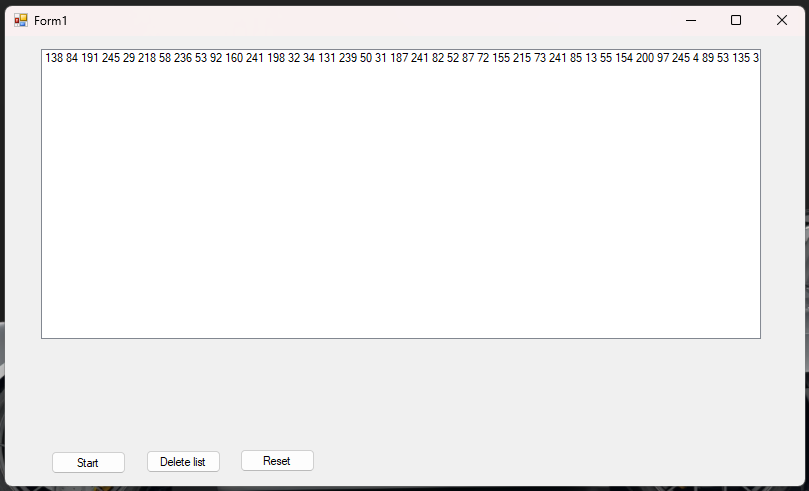
\includegraphics[width=0.7\linewidth]{tesztalkalmazas}
	\caption[Teszt alkalmazás]{Teszt Windows Forms alkalmazás}
	\label{fig:tesztalkalmazas}
\end{figure}

Aztán következhetett a szenzor tesztelése. Először egy fehér lapon próbálkoztam amire kisbetűmérettel volt rá írva pár betű, viszont valamiért nem kaptam egy szép képet, ezért elkezdtem mozgatni a szenzort és rájöttem, hogy a fókusz távolság nem volt a megfelelő. Így azt kellett finom hangolnom, egyszerű kártya lapokat használtam, hogy megtaláljam a megfelelő távolságot. Miután sikerült beállítanom a kellő távolságot a papírtól, elkezdtem kinyerni a szenzorból a képeket. Megírtam hozzá a teszt alkalmazást amivel megjelenítem, hogy mit lát a szenzor, és nagyon nagy örömömre sikerült képet kinyernem a szenzorból.
\begin{figure}[th!]
	\centering
	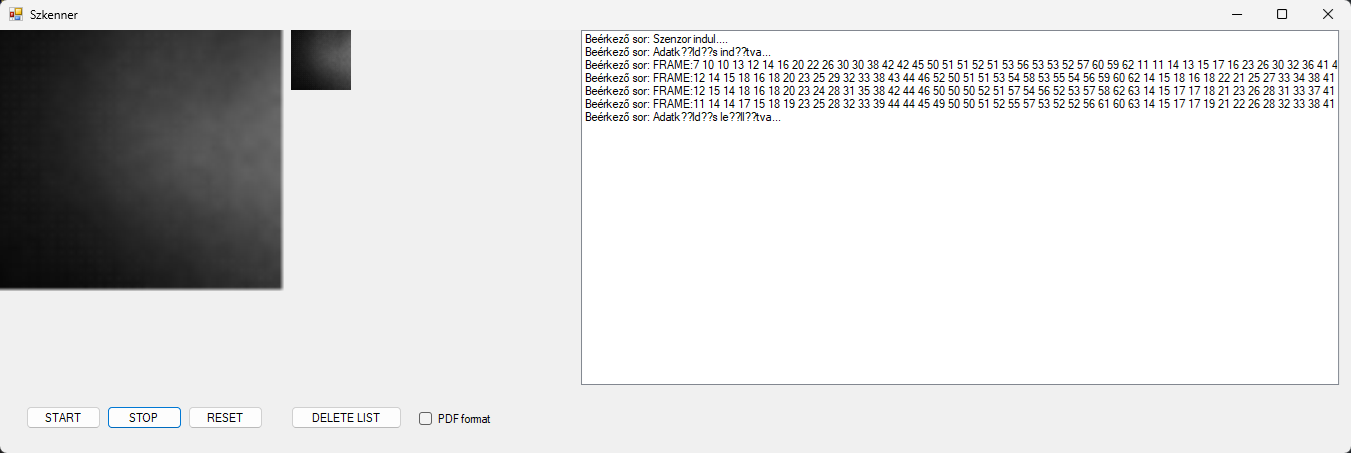
\includegraphics[width=1\linewidth]{tesztalkalmazas2}
	\caption[Teszt2]{Továbbfejlesztett teszt alkalmazás}
	\label{fig:tesztalkalmazas2}
\end{figure}

Végezetül a motorok teszteléséhez half-step módot próbáltam alkalmazni, viszont a bipoláris léptető motorral nem működött, ezért ott a Stepper könyvtárat kellett használnom. Közben felmerült egy olyan probléma, hogy az általam használt motorvezérlő elromlott ezért egy másikat kellett beszerelnem. Ezután jöhetett a szkennerbe való beszerelés, amelyben Geda Gábor tanár úr segített nekem. Így született meg \aref{fig:scanner_prototype}. számú ábrán látható szkenner.
	\begin{figure}[th!]
		\centering
		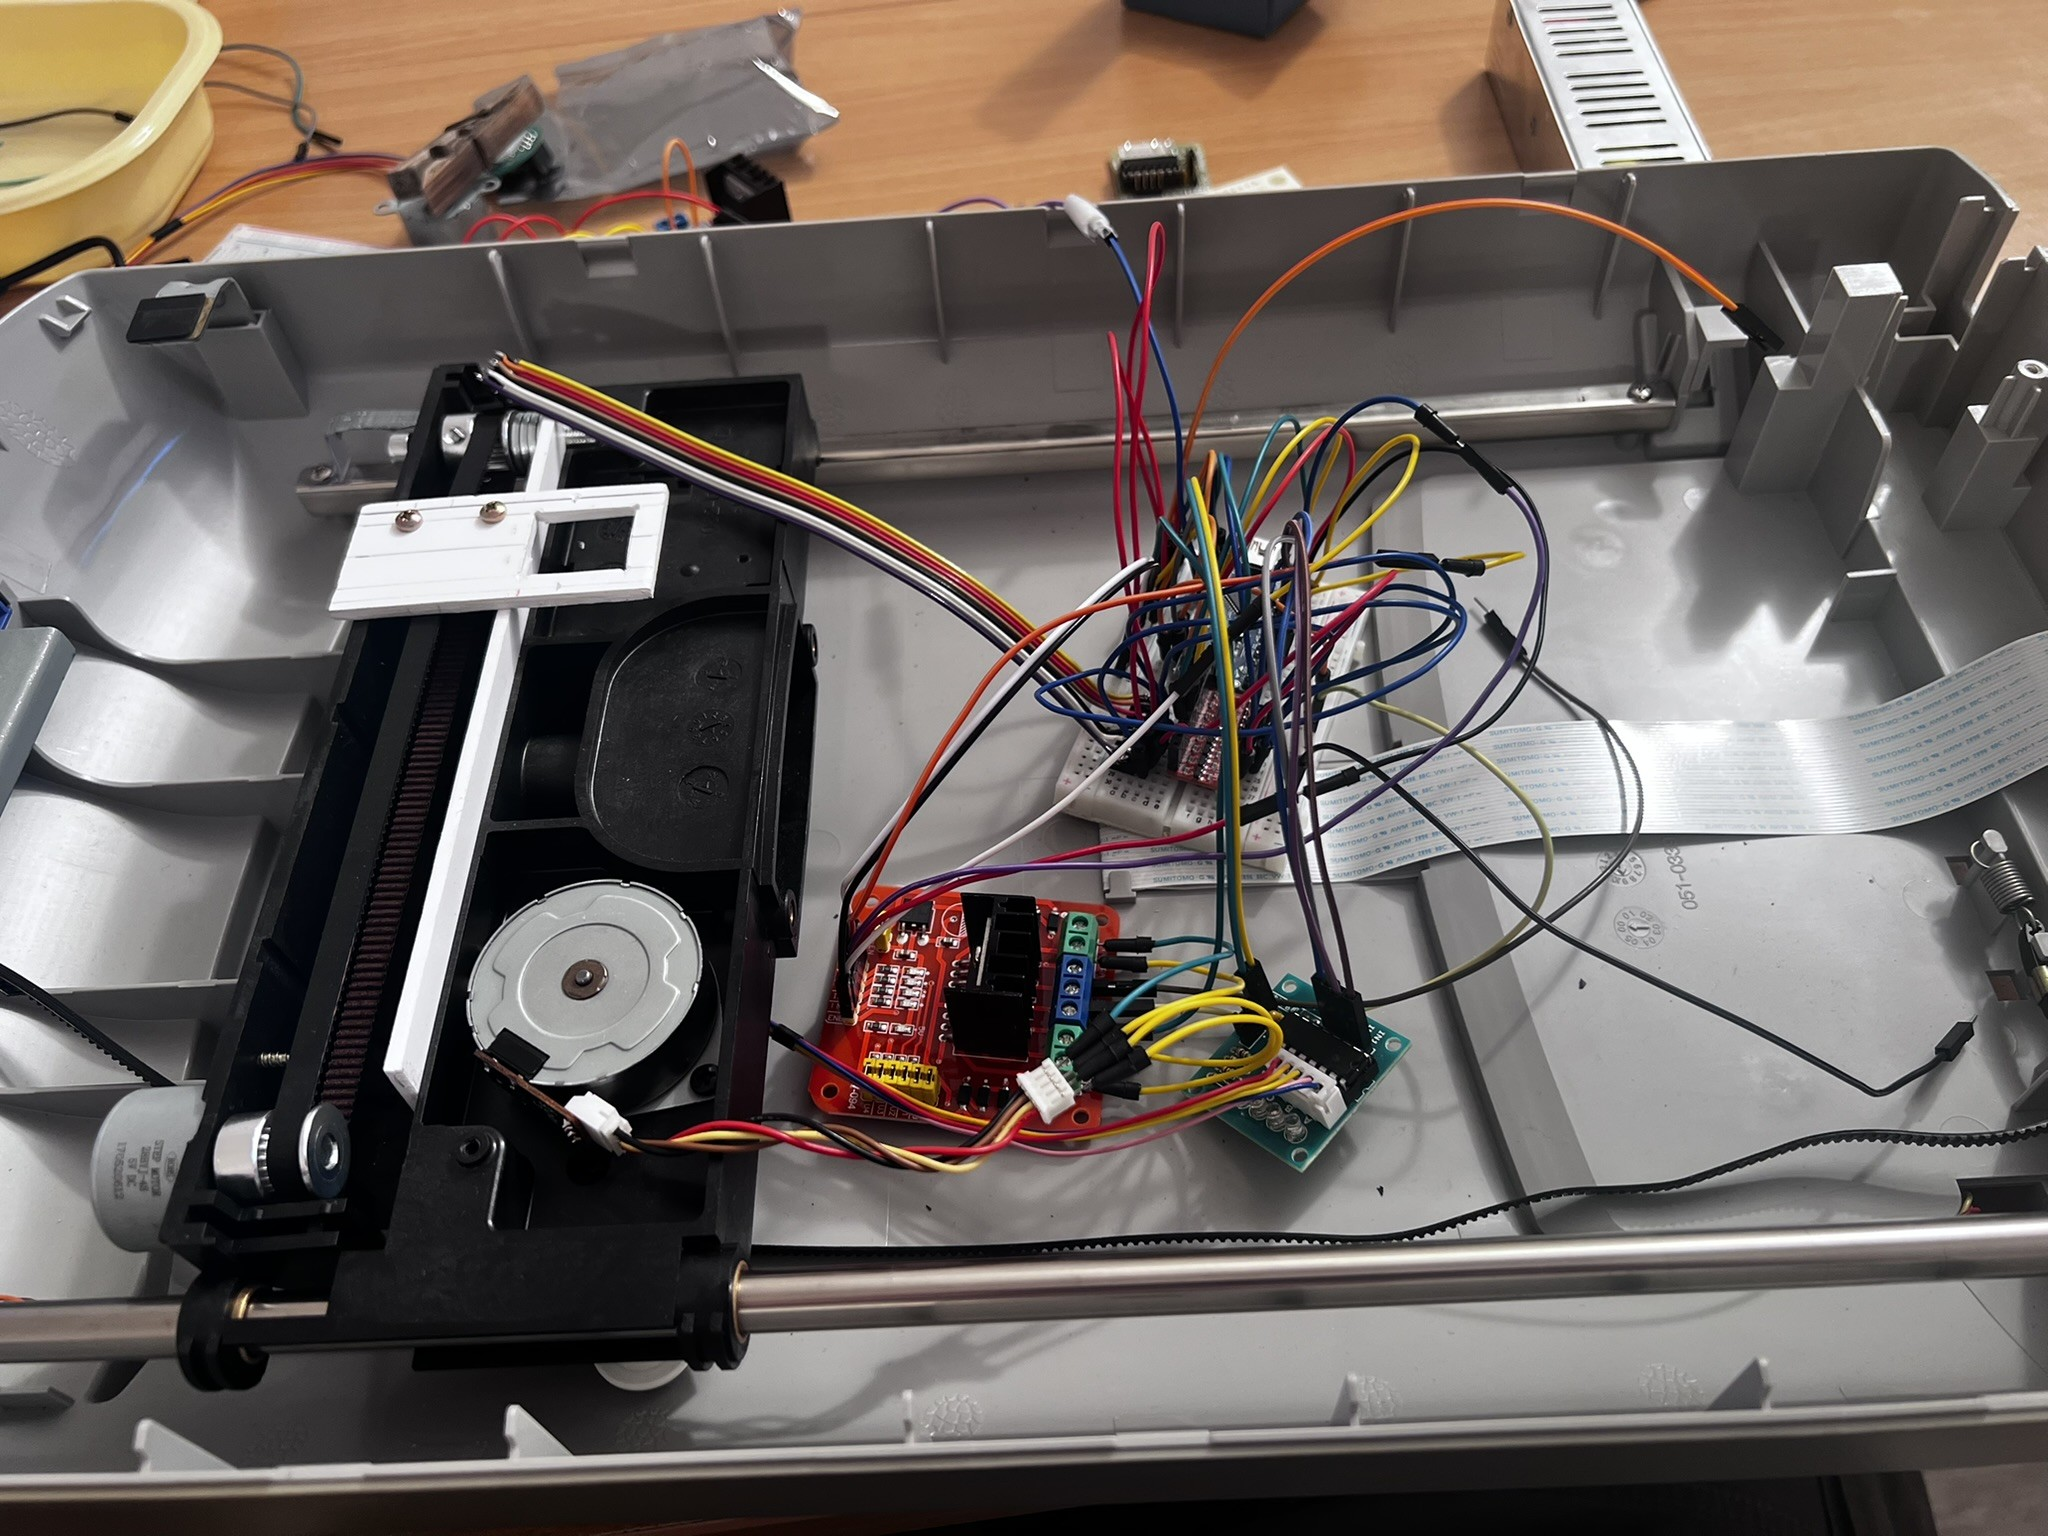
\includegraphics[width=0.7\linewidth]{scanner}
		\caption[Összeépített szkenner]{Összeépített szkenner}
		\label{fig:scanner_prototype}
	\end{figure}
\pagebreak

Ezután a helyére kerültek a fénykapuk is amikkel a kezdőpozícióját tudtam megállapítani a szenzornak. Két kis zászlót készítettünk amik a sínen valamint a szenzornál helyezkednek el, ezáltal ha a zászló be megy az infravörös érzékelők közé, jelez, hogy megérkezett a kezdőállapotba. Felmerült közben sajnos egy olyan probléma, hogy az Arduino tápja nem bírta el a terhelést, ezért be kellett építeni egy külön 5\,V-os tápot az unipoláris motor működéséhez. Végezetül összeállt a végleges szkenner amelyet \aref{fig:finishedscanner}. számú ábrán láthatunk.
\begin{figure}[th!]
	\centering
	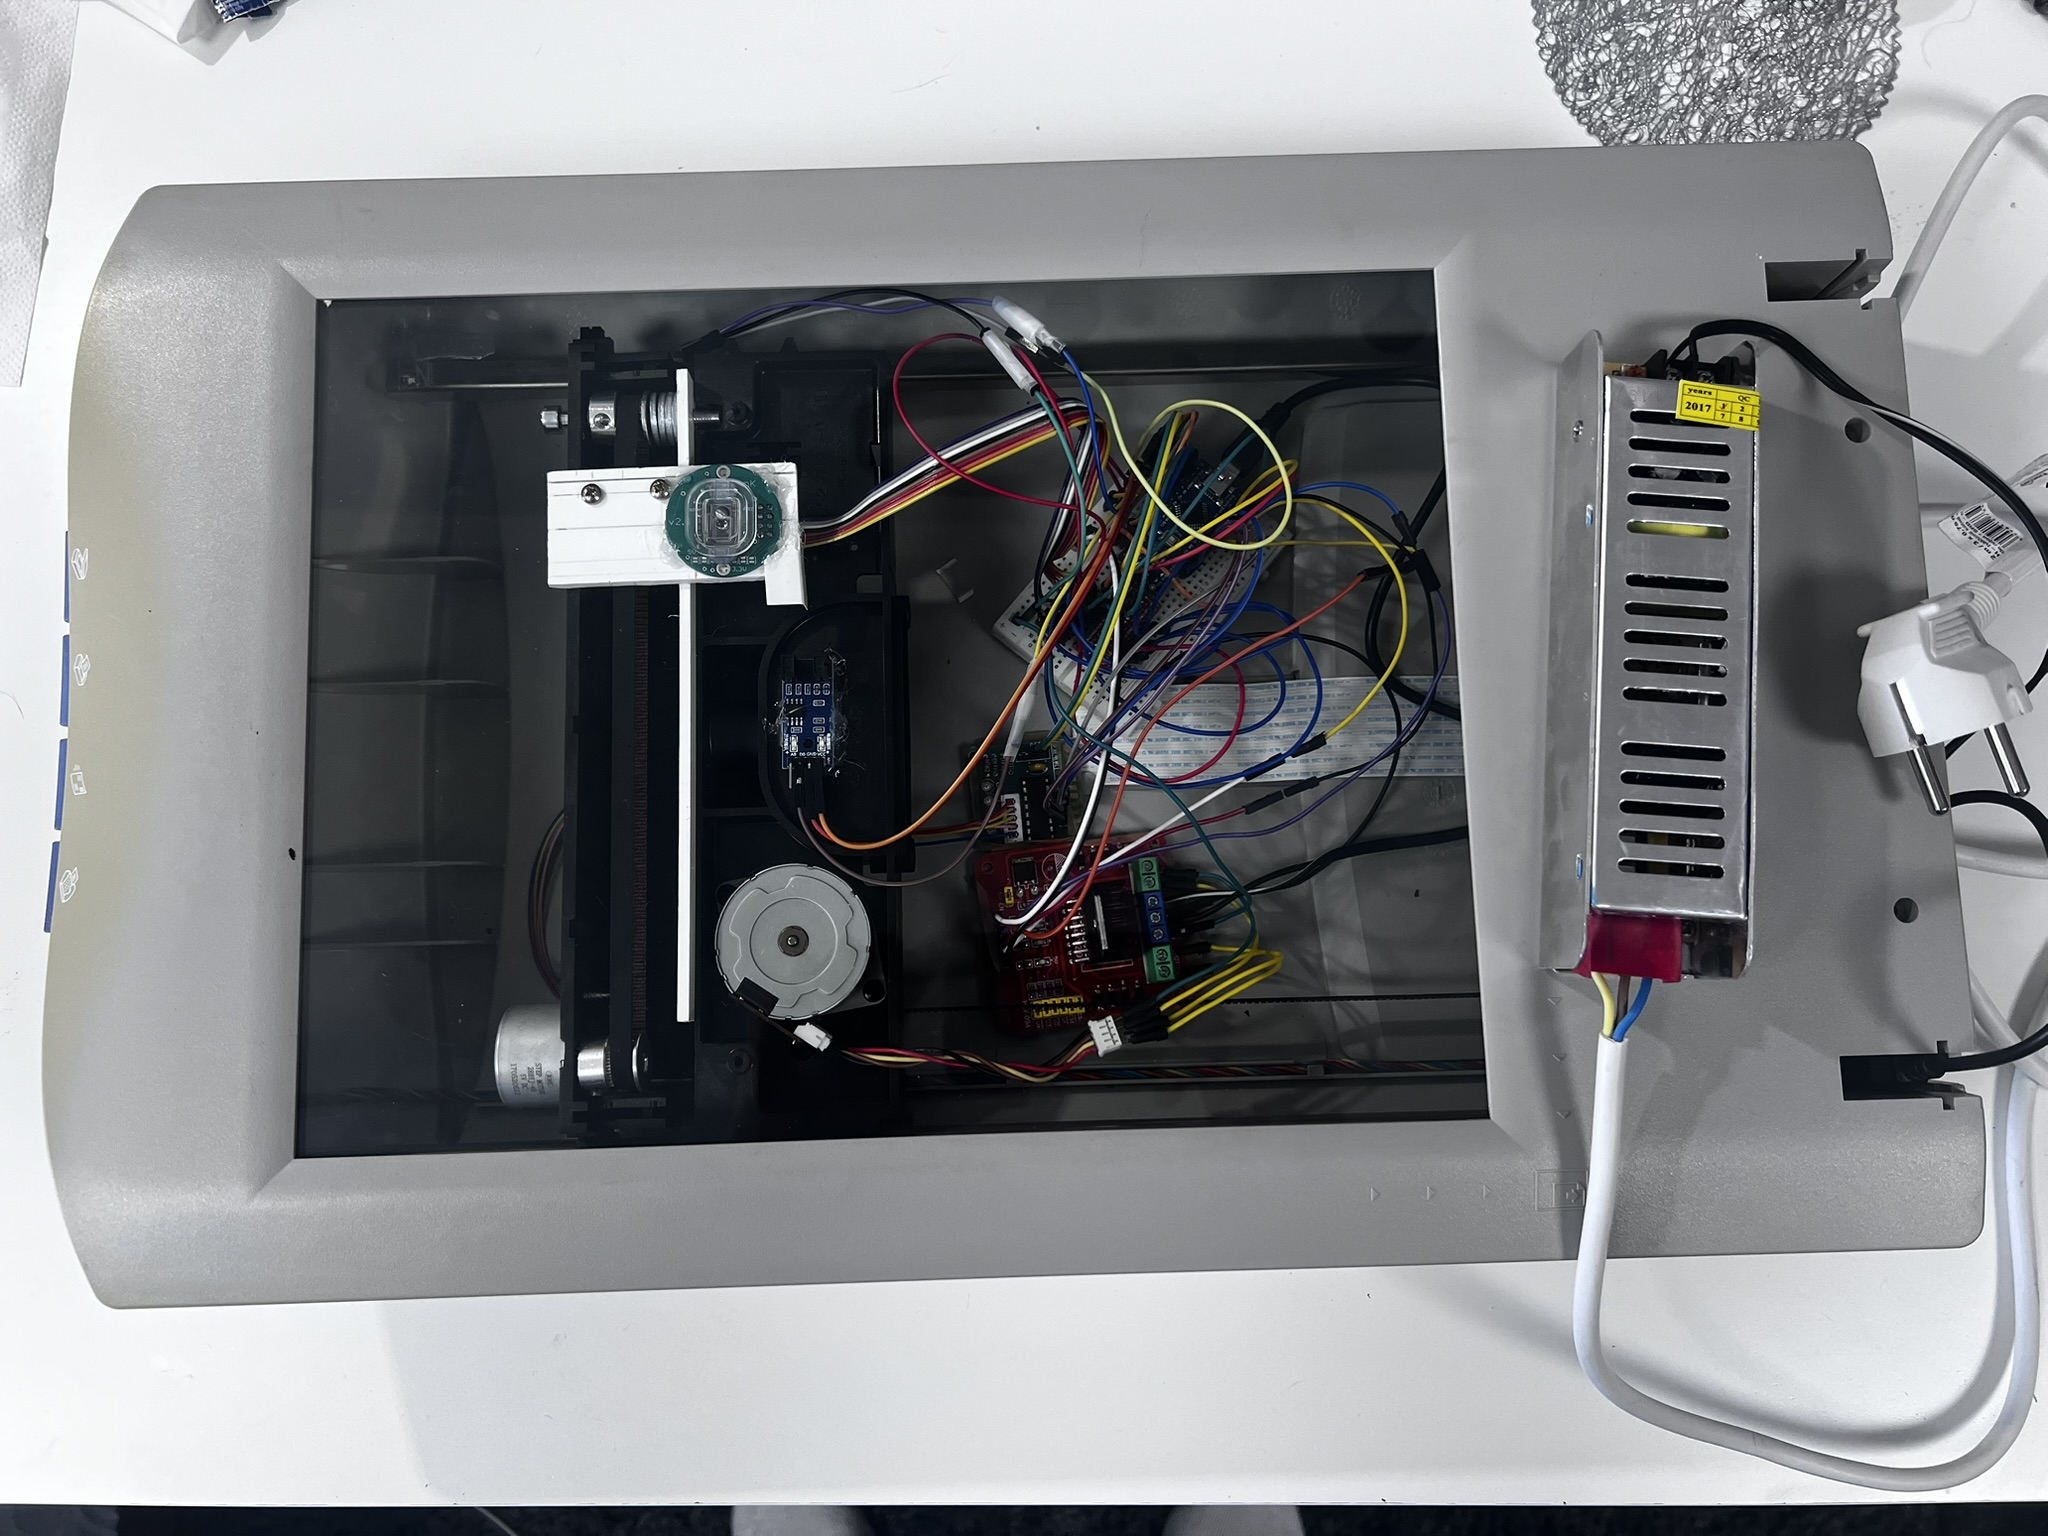
\includegraphics[width=0.7\linewidth]{finished_scanner}
	\caption[Végleges szkenner]{Végleges szkenner}
	\label{fig:finishedscanner}
\end{figure}

\chapter*{Összegzés}
Összességében a szakdolgozatom elkészítése közben nagyon sok új elektronikai és programozási tapasztalatra tettem szert. A projekt alatt nem csak az Arduino környezetet értettem meg jobban, hanem sok hardveres eszköz működését is jobban megértettem, például a léptetőmotorok vagy maga a szenzor. A projekt során még azt is megtanultam, hogy hogyan lehet a szoftver és hardver működését összehangolni. Igaz, hogy sajnálatos módon egy olyan szenzort sikerült beszereznem, amely a fókusztávolságból adódó hardveres korlátok miatt nem képes jó minőségű képet alkotni.

Ez a szkenner egy egyszerű fekete-fehér képolvasó, viszont jó alapot biztosít a további fejlesztésekhez, mint például:
\begin{itemize}
	\item A jelenlegi színtelen szkennert 3 darab LED-el tovább lehetne fejleszteni egy színes szkennerré.
	\item A mostani változat sajnos csak egy kis részt tud beolvasni, ezért az is egy továbbfejlesztési gondolat lehetne, hogy egy teljes A4-es lapot beolvasson.
	\item Esetleg az is szóba jöhetne, hogy Wi-Fi-n keresztül telefonra kapnánk meg a beolvasott dokumentumot.
\end{itemize}
\vspace*{2cm}
Köszönet nyilvánítás: 

Külön köszönettel tartozom Dr. Geda Gábor tanár úrnak, aki az egész projekt során végig rendkívül segítőkész és támogató volt. Az iránymutatásai és tanácsai nélkül a szakdolgozatom nem valósulhatott volna meg ilyen formában.
\addcontentsline{toc}{chapter}{Összegzés}
\chapter*{Ábrajegyzék}
\begin{itemize}
	\item \ref{fig-arduinofamily}. ábra: \emph{\url{https://predictabledesigns.com/wp-content/uploads/2017/10/HeroImage.png}}
	\item \ref{fig:atmega328p-pu}. ábra: \emph{\url{https://techfun.hu/wp-content/uploads/2017/09/11.jpg}}
	\item \ref{fig:arduino-nano-pinout}. ábra: \emph{\url{https://www.makerguides.com/wp-content/uploads/2020/10/arduino-nano-pinout-768x603.png}}
	\item \ref{fig:adns9800base}. ábra: \emph{\url{https://www.sicstock.com/cdn/shop/products/551554.jpg?v=1544514465}}
	\item \ref{fig:adns9800}. ábra: \emph{\url{https://tinyurl.com/2z4zn3d9}} 
	\item \ref{fig:szintilleszto}. ábra: \emph{\url{https://www.elektrobot.hu/items/3607_1.webp}}
	\item \ref{fig:mitsumi-stepping-motor-m42sp-4np}. ábra: \emph{\url{https://www.picmicrolab.com/wp-content/uploads/2014/04/MITSUMI-Stepping-Motor-M42SP-4NP.jpg}}
	\item \ref{fig:stepper-motors-half-step}. ábra: \emph{\url{https://www.orientalmotor.com/images/stepper-motors/stepper-motors-half-step.jpg}}
	\item \ref{fig:28byj-48-modul-uln2003}. ábra: \emph{\url{https://www.hwlibre.com/wp-content/uploads/2024/10/28byj-48-circuito.jpg}}
	\item \ref{fig:mh-infrared-speed-sensor-module}. ábra: \emph{\url{https://einstronic.com/wp-content/uploads/2020/11/MH-Infrared-Speed-Sensor-Module-1.jpg}}
	\item \ref{fig:circuit}. ábra: \emph{Saját ábra a \url{https://www.circuit-diagram.org/} segítségével}
	\item \ref{fig:tesztalkalmazas} .ábra: \emph{Saját ábra}
	\item \ref{fig:tesztalkalmazas2} .ábra: \emph{Saját ábra}
	\item \ref{fig:scanner_prototype} .ábra: \emph{Saját ábra}
	\item \ref{fig:finishedscanner} .ábra: \emph{Saját ábra}
\end{itemize}
\addcontentsline{toc}{chapter}{Ábrajegyzék}
\begin{thebibliography}{9}
\addcontentsline{toc}{chapter}{\bibname}
\bibitem{szakdolgozat} Github link a szakdolgozathoz: \url{https://github.com/Bmate2/SZAKDOLGOZAT}
\bibitem{arduino} Arduino: \url{https://www.arduino.cc/en/Guide/Introduction}
\bibitem{whatisanarduino} What is an Arduino: \url{https://learn.sparkfun.com/tutorials/what-is-an-arduino/all}
\bibitem{arduinouno} Arduino UNO: \url{http://dx.doi.org/10.6084/m9.figshare.11971794.v1}
\bibitem{arduinonano} Arduino Nano: \url{https://docs.arduino.cc/hardware/nano/}
\bibitem{visual-studio} Microsoft Visual Studio: \url{https://visualstudio.microsoft.com/}
\bibitem{github} Github: \url{https://github.com/}
\bibitem{adns9800} ADNS-9800 adatlap:\url{https://datasheet.octopart.com/ADNS-9800-Avago-datasheet-10666463.pdf}
\bibitem{adns9800_buy} ADNS-9800 vásárlás: \url{https://www.tindie.com/products/citizenjoe/adns-9800-motion-sensor/}
\bibitem{adns9800_2} ADNS-9800 tutorial get travel distance: \url{https://www.instructables.com/Arduino-Tutorial-ADNS-9800-Laser-Mouse-Traveled-Di/}
\bibitem{adns9800_3} ADNS-9800 5\,V mód aktiválása: \url{https://forum.arduino.cc/t/using-avago-adns9800/292172/2}
\bibitem{szintilleszto} Logikai szintillesztő modul: \url{https://www.elektrobot.hu/termek.php?filename=3607.html&i=3607}
\bibitem{serial} Soros kommunikáció: \url{https://docs.arduino.cc/language-reference/en/functions/communication/serial/}
\bibitem{motorvezerlok} Léptető motorok: \url{https://docs.arduino.cc/learn/electronics/stepper-motors/}
\bibitem{l298n} L298N motorvezérlő: \url{https://techfun.hu/termek/l298n-vezerlomodul-dual-h-bridge-v2-0-motorkerekparokhoz/?gad_source=1}
\bibitem{stepper} Arduino Stepper könyvtár: \url{https://docs.arduino.cc/libraries/stepper/}
\bibitem{bicubic_video} Bicubic Interpolation by Computerphile: \url{https://www.youtube.com/watch?v=poY_nGzEEWM}
\bibitem{bicubic_wikipedia} Bicubic Interpolation from wikipedia: \url{https://en.wikipedia.org/wiki/Bicubic_interpolation}
\bibitem{bicubic} Bicubic Interpolation: \url{https://cloudinary.com/glossary/bicubic-interpolation}
\bibitem{catmull-rom_spline} Catmull-Rom Spline: \url{https://en.wikipedia.org/wiki/Centripetal_Catmull%E2%80%93Rom_spline}
\bibitem{image_upscale} Kép nagyítás Bikubik interpolációval: \url{https://medium.com/@amanrao032/image-upscaling-using-bicubic-interpolation-ddb37295df0}
\bibitem{winforms} Windows Forms: \url{https://learn.microsoft.com/hu-hu/dotnet/visual-basic/developing-apps/windows-forms/}
\bibitem{listbox} Listbox osztály: \url{https://learn.microsoft.com/en-us/dotnet/api/system.windows.forms.listbox?view=windowsdesktop-9.0}
\bibitem{arduino_latex} \LaTeX\ Arduino stílus fájl: \url{https://github.com/trihedral/ArduinoLatexListing}
\bibitem{bitmap.class} Bitmap osztály: \url{https://learn.microsoft.com/en-us/dotnet/api/system.drawing.bitmap?view=windowsdesktop-9.0}
\bibitem{matrixToBitmap} Mátrix átalakítása Bitmap képpé: \url{https://swharden.com/csdv/system.drawing/array-to-image/}
\bibitem{lockbit} Bitmap.LockBits használata: \url{URLhttps://learn.microsoft.com/en-us/dotnet/api/system.drawing.bitmap.lockbits?view=windowsdesktop-9.0}
\bibitem{fastpixeloperation} Lockbit vs SetPixel: \url{https://www.codeproject.com/Articles/617613/Fast-Pixel-Operations-in-NET-With-and-Without-unsa}
\bibitem{rectangle} Rectangle osztály: \url{URLhttps://learn.microsoft.com/en-us/dotnet/api/system.drawing.rectangle?view=net-9.0&viewFallbackFrom=windowsdesktop-9.0}
\bibitem{marshal.copy} Marshal Copy metódus: \url{https://learn.microsoft.com/en-us/dotnet/api/system.runtime.interopservices.marshal.copy?view=net-9.0}
\bibitem{aspose.word} Aspose.Words nuget csomag a dokumentum mentéshez:  \url{https://www.nuget.org/packages/aspose.words}
\end{thebibliography}

% Aláírt, szkennelt nyilatkozat beillesztése a szakdolgozat végére
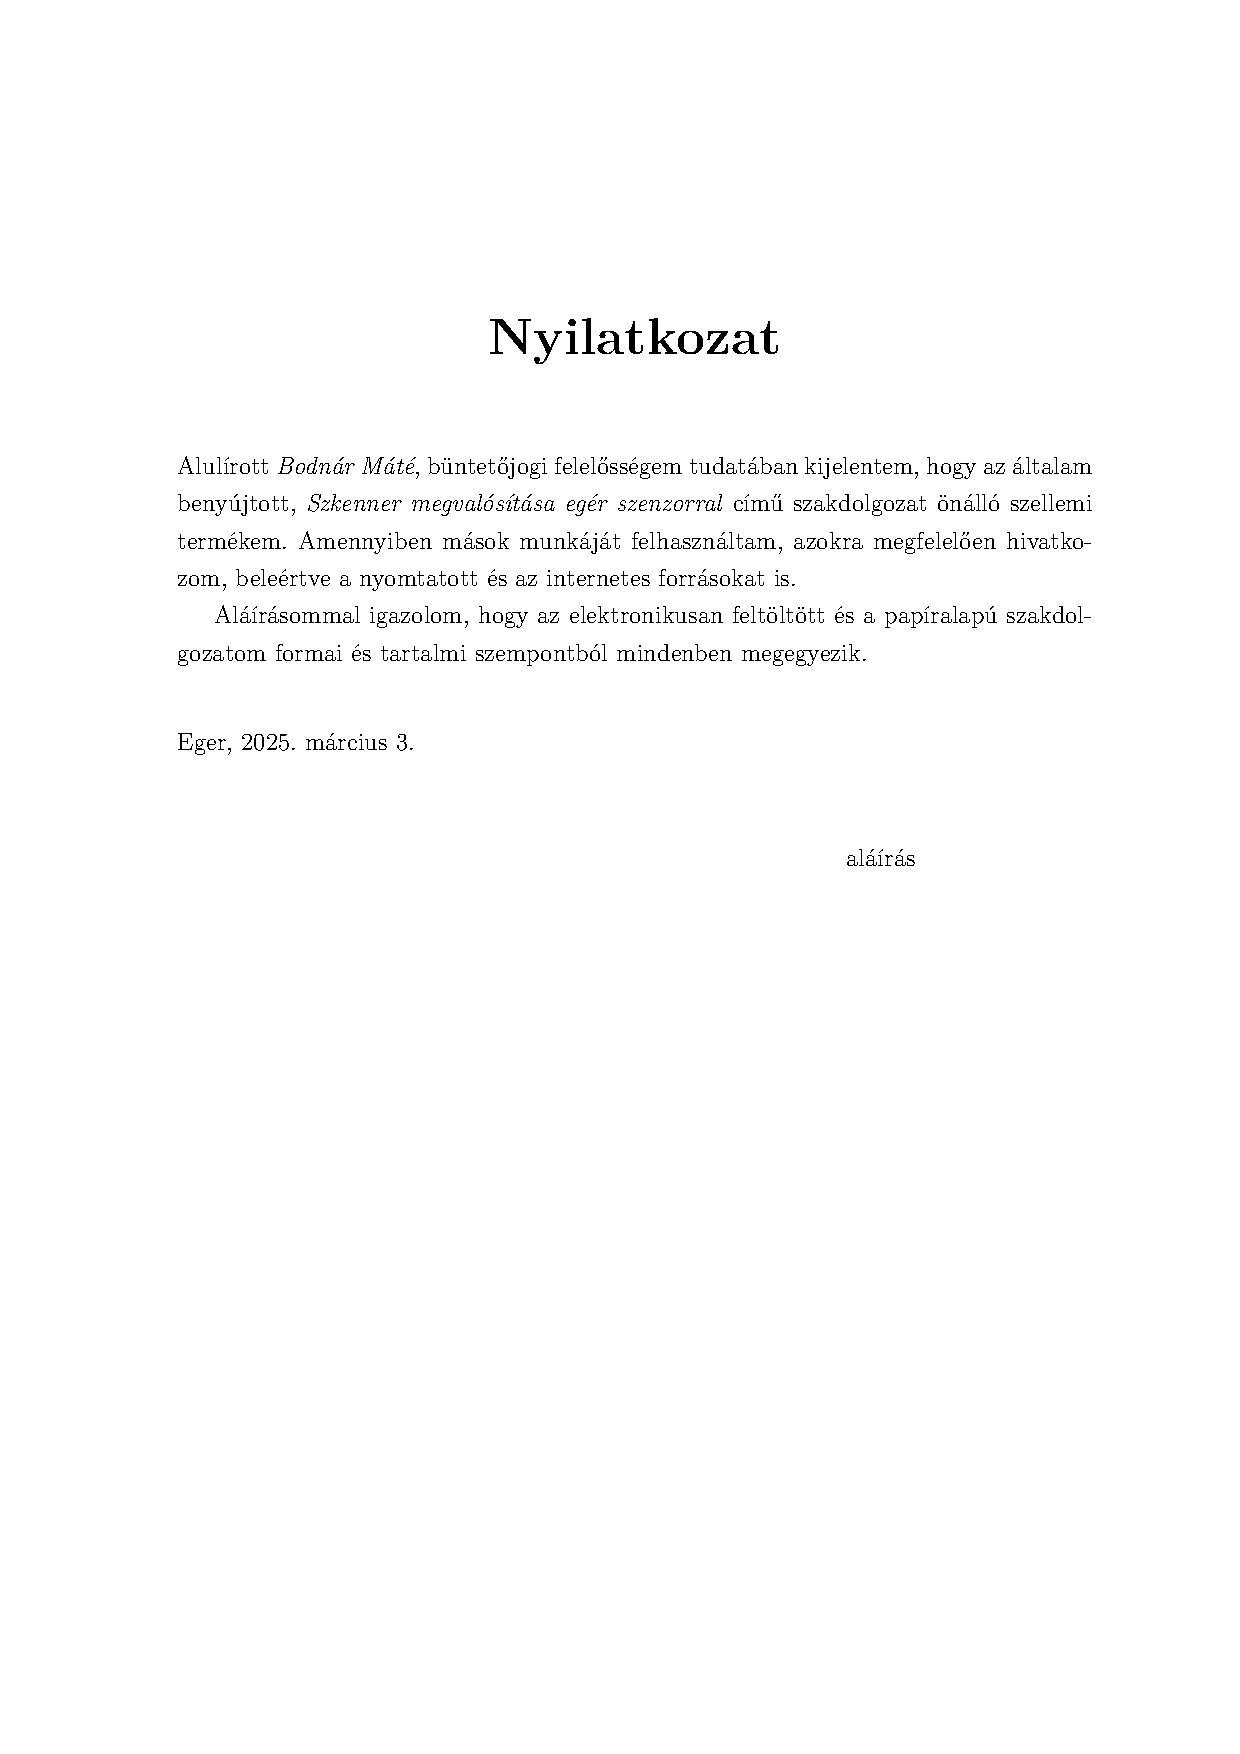
\includepdf{Nyilatkozat/nyilatkozat.pdf}

\end{document}
